\documentclass[10pt]{book}
\usepackage{NotesTeXV3,lipsum}
% tikz is in the style file
\usetikzlibrary{calc, angles, quotes}
\usetikzlibrary{quantikz2}
\newcommand{\AxisRotator}[1][rotate=0]{%
    \tikz [x=0.25cm,y=0.60cm,line width=.2ex,-stealth,#1] \draw (0,0) arc (-150:150:1 and 1);%
}
\usepackage{pgf}
\usepackage{pgfmath}
\usetikzlibrary{shapes.geometric, math}

\usepackage{imakeidx}
\makeindex

\title{
    Materials for the simulation of quantum system behavior on quantum computer}
\author{Hyunseong Kim}
\emailAdd{qwqwhsnote@gm.gist.ac.kr}

\begin{document}
\maketitle
\newpage
\pagestyle{fancynotes}

\section*{Preface}

This document is a cheet-sheet and proof-notes about 
quantum simulation on quantum computer, especially, in gate model.
If you know basic postulations and concepts of quantum computers and you want to implement the simulation
of the given quantum system, it might be helpful. 

Mainly focusing on Product-formula method and its optimization topics. 
They are basic materials for any kinds of quantum simulation and my Bachelor thesis subject.
The formalization part is a basic materials for the product formula implementation
minimizing errors on the formulation steps.
The mathematical background of the evolution circuit and their representations were dicsussed.
Optimization part is about the optimize the evolution circuit by using various techniques.
In the practical part, we review the many practical techniques using quantum 
computer and their simple implementations. 
The modeling of the single-particle system, adiabatic process implementation, 
VQE introduction are dicussed.
In the further topics part, we reviewed the advanced topics. 
Using 1 dim particle simulator, we dicussed about tunneling phanomenon and their 
simulation in quantum computer.
Material modeling and physcial properties simulation in many-body physics,
binary optimization in quantum computer briefly reviewed.

Written programs and algorithm implemnetations are also provided with refering repositories.
In appendix, step by step example of simulation and measurement 
using some popular quantum frameworks;Qiskit, Pennylane, D-Wave et cetra.


Most contents are related with author's studies and research in the course of Quantum Graduate School internship
established by 8 university. Thanks for Dr. Kim(GIST), Dr. Yee(GIST) and Dr. Choi(Korea).

\begin{itemize}
    \item 2023 Summer Special Internship, held by Korea university
    \item Bachelor research internship on Quantum Field and Gravitation Lab of GIST
    \item Bachelor research internship on Computational Material Lab of GIST
\end{itemize}

Abbrevations

\begin{itemize}
    \item QC: Quantum computation
    \item CC: Classcial computation
\end{itemize}

\newpage

\part{Simulation of Quantum system}
\chapter{Formalization and Evolution}

\section{How does quantum computer simulate system?}

A quantum system basically lies in continuous Hilbert space of normalized complex functions, \textit{wave function} or \textit{quantum field}.
However, common universal quantum computing model; \textit{circuit model}, is not a continuous quantum model. 
It is a discrete computation model. There are some continuous computation model in quantum computer, such as \textit{adiabatic model}. 
However, in this document we will focus on the circuit model and the adiabatic model would be treated in separated application chapter.
Therefore, if we want to simulate a given quantum system, 
first thing to do is a discrete formalization to run on the gate model system.

The discretization is not a new concept in quantum computation. 
We can simulate various quantum systems in classic computation model already, 
and the implementation of the simulation on the system requires appropriate discretization techniques.
The common notation and techniques of the quantum computation were adopted from classic computation technique. 
The differences are efficiency of computation and existence of the model. 
Many quantum systems do not have an any approximation model.
For example, in condensed matter physics, 
Ising, and Hubbard Hamiltonian have been frequently used to describe the spin system of solid material.
Even we just increase the dimension or lattice site, the problems become too complicated to solve or to compute 
their behavior\footnote{For Ising, only 1 and 2 dimension cases are exactly solvable, and the further dimensions have no solution.}.
However, quantum computer could simulate their behavior efficiently, comparing to the computational techniques
in classic computers. 
In addition, even the most complicated system was given, at least, 
we can try the basic techniques by simulating time-evolution.

Then, what does the discrete model affect the computation and the modeling of the problem?.
Considering a differential equation. All we do in quantum mechanics is getting solutions of the given differential equations.
We want to approximate the solution, $f(x)$, of the equation, 
$D(x, f, f', \dots) = 0$, 
with given initial or boundary conditions, $(x_0, f(x_0))$.
We first discrete the region of consideration with $\Delta x$ and approximate 
the next points start from the initial value to the target value.
This is called by \textit{Euler method}. 

\begin{align}
    (x_0, f(x_0)) \\
    x_i = x_{i-1} + \Delta x \\
    f(x_i) = f(x_{i-1}) + \sum \lambda_n f^{(n)}(x_i) (\Delta x)^n
\end{align}

There are several techniques to update the point value in each step, but the details are not a consideration in here, 
see numerical analysis textbook for the details\footnote[1]{Cheney, E Ward, or Burden et al are famous.}.
The gate model simulation of quantum system is exactly same with the above discrete approximation. 
We update the intermediate state until we reach the state we want to observe.
When we want to simulate the evolution of the system, first thing to do is preparing the initial system configuration, and 
we can obtain the target state by applying several evolution operators with evolution time, $\Delta t$.

These are main focus of the material. 
The quantum computer provides for us to simulate the complex systems in many areas 
not only for physics, but also for many engineering, especially computer science.
We already have general frameworks to manipulate the operation, preparation,
and dynamics of the quantum states. 
However, the exact process to simulate the given quantum state 
is still remained for us.

\begin{enumerate}
    \item How to formulate \textit{time-evolution} in quantum computing language?
    \item How to implement the evolution process?
    \item What error could be happened during the operation?
    \item How to model a specific system to simulate with quantum computer?
\end{enumerate}

There are many techniques and requirements for researchers and engineers to know.
Thus, in here, we will overlook those techniques
from solid mathematical backgrounds to programming implementation.

\section{Time evolution operator of the system}

We start from the simplest situation; a time independent Schr$\ddot{\mbox{o}}$dinger equation,

\begin{equation*}
    i \hbar \frac{\partial }{\partial t} | \psi \rangle = H | \psi \rangle
\end{equation*}

In Schr$\ddot{\mbox{o}}$dinger picture, where the operators are time dependent,
We can express a solution of $|\psi(t) \rangle$ with unitary operator, $U$,
\begin{equation}
    \label{eq:time_inde_sol}
    |\psi(t)\rangle = U(t) | \psi(0)\rangle 
\end{equation}

What we have at the initial stage were an initial state and the given Hamiltonain.
From the information, we have to get a $U(t)$ operator for simulate
the dynamics of the given system.
The solution of Eq (\ref{eq:time_inde_sol}) is achieved easily 
if the $H$ has no time dependency\footnote{
    In general, the solution is never gone like the Eq (\ref{eq:time_inde_sol}). 
    We will see it in a further section.}.

\begin{equation}
    U(t) = \exp( -i \frac{1}{\hbar} (H) t)
\end{equation}

A more precise notation is $U(t_i, t_f)$ which indicates the initial time and final time.
With the notation, the $U(t)$ is $U(0, t)$.
We call it as a time-propagator\footnote{
    In mathematics, such propagator is a green function of solution of differential or integral equations.
    $G(s_n, t_n | s_0, t_0) = U(t_n, t_0)$
}
Here is why the gate model is called a discrete computation model.
It is because we cannot directly implement the such general time-propagator 
per each system. Only thing we can manipulate is just an approximation 
of the propagator with basic block gates. 
Fortunately, the universal gate set to represent approximate all unitary operator
is well investigated. See \textit{Solovay-Kitaev theorem}.
\index{Solovay!Solovay-Kitaev theorem}
\index{Kitaev!Solovay-Kitaev theorem}


\begin{definition}\textbf{Unitary approximation}
    For a given unitary gate, $U(t)$, 
    approximation of $U(t)$ is a constructing an $U'(t)$ gate 
    which consist of the universal gate set of the quantum machine,
    such that minimize the next,

    \begin{equation}
        \max\left(|U(t) - U'(t)|\right)
    \end{equation}
\end{definition}

%---------------------------------

\begin{marginfigure}
    \centering
    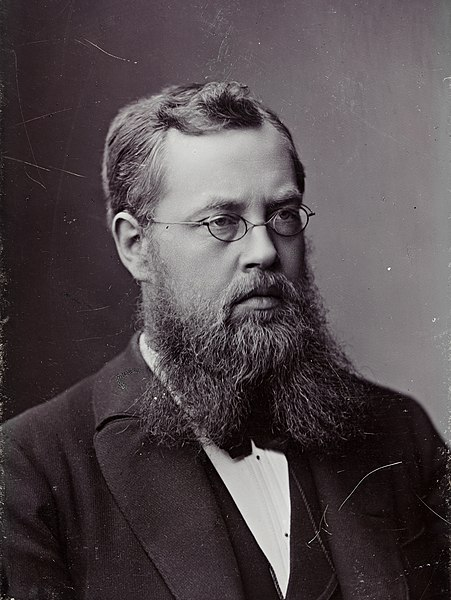
\includegraphics[width=0.6\textwidth]{media/picture_Sophus_Lie.jpg}
    \caption{Sophus Lie}
    \label{fig:sopus_lie_picture}
\end{marginfigure}
\index{Lie}
\index{Sophus Lie}

Then, what we need? What does the operator mean inside of exponential?
It is called exponential mapping of operator, and 
it plays a key concept of time-evolution in quantum mechanics.
The major properties and definiton were first investigated by \textit{Sophus Lie} with his research on continuous group and 
differential geometry.
It has tremendous interesting properties and applications in both physics and mathematics.
However, in here, we only look up 
the operator map for evolution implementation in finite matrix group.

\subsection{Exponential Map}

\begin{definition}{\textbf{Operator exponential}}
    \index{Operator Exponential}
    \begin{equation}
        \exp(\hat{X}) = \sum_{k=0} \frac{1}{k !} \hat{X}^k
    \end{equation}
\end{definition}

The map is converges $\forall X \in \mathbf{M}_{n}(\mathbb{C})$.

\begin{theorem} \textbf{Properties of Exponential Map}
    \begin{itemize}
        \item $e^X$ is a continuous function.
        \item $e^0 = I$
        \item $(e^X)^\ast = e^{X^\ast}$
        \item $e^X$ is always invertible, and $(e^X)^{-1} = e^{-X}$.
        \item $e^{(a+b)X} = e^{aX} e^{bX}$.
        \item If $[X, Y] = 0$, $e^{X+Y} = e^{X}e^{Y} = e^{Y}e^{X}$.
        \item $\forall M \in \text{GL}(n; \mathbb{C}), e^{M X M^{-1}} = M e^{X} M^{-1}$. 
    \end{itemize}
\end{theorem}

If $\hat{A}$ was a digonal matrix, then the next relationship hold.

\begin{equation*}
    A = \begin{bmatrix}
        \lambda_1 & 0 & \dots & 0 \\
        0 & \lambda_2 & \dots & 0 \\
        \vdots & 0 & \ddots & \vdots\\
        0 & 0 & \cdots & \lambda_n
    \end{bmatrix},
    e^A = \begin{bmatrix}
        e^{\lambda_1} & 0 & \dots & 0 \\
        0 & e^{\lambda_2} & \dots & 0 \\
        \vdots & 0 & \ddots & \vdots\\
        0 & 0 & \cdots & e^{\lambda_n}
    \end{bmatrix}
\end{equation*}

In general not only for the digonal matrix, 
the exponential map preserves the eigenvectors of the original matrix.

\begin{exercise}
    For an eigen vector, $\mathbf{v}$, of the given matrix, $X$, with eigenvalue, $\lambda$,

    \begin{equation}
        X \mathbf{v} = \lambda \mathbf{v}
    \end{equation}

    Show that 

    \begin{equation*}
        e^X \mathbf{v} = e^\lambda \mathbf{v}
    \end{equation*}
\end{exercise}

In general case, we decompose the Hamiltonian as sum of local terms,
and the time as sum of many intermediate steps.
These slicing allow us to analysis the dynamics of the system evolution
in specific local region or local time. 
First, the time slicing is not different with usual exponential function.
The time-propagator from time $t_0$ to $t_n$ can be decomposed to 
$n$ intermediate step propagators,

\begin{eqnarray*}
    U(t_n, t_0) &= U(t_0 + \Delta t, t_0) U(t_0 + 2\Delta t, t_0 + \Delta t) \cdots U(t_n, t_n - \Delta t) \\
                &= \Pi_{i=0}^{n-1} U(t_{i+1}, t_i)\\
                &= \Pi_{i=0}^{n-1} \exp \left( - i \Delta t H\right)\\
                &= \exp \left( - i (t_n - t_0) H\right)\
\end{eqnarray*}

However, decomposition with local Hamiltonian, $H = \sum_k H_k$ yields 
a problem. The non-commuting terms in $\sum_k H_k$ makes an error in the expotential map.

\begin{align*}
    [H_i, H_k] \neq 0\\
    e^{H_i + H_k} \neq e^{H_i} e^{H_k} \, \text{ or } \, e^{H_k} e^{H_i}
\end{align*}

Major problem arises in here. 
Since, we cannot directly implement the given evolution gate, 
but just applying sequential local term does not yield
the correct gate. The problem would be investigated in the following 
subsection. 

\subsubsection{Pauli matrix and exponential}

Before, we move to the non-commuting problem. 
Let us see basic properties of Pauli matrices as a basis set of matrix space.
In the above paragraph, we read the Hamiltonian could be decomposed 
into several local Hamiltonians. 
Mostly, we decompose them with Pauli matrices.
Since, Pauli matrices have good properties to decompose 
the general Hamiltonian. 

\begin{definition}\textbf{Pauli matrices}
    \index{Pauli matrices}
    \begin{equation}
        \sigma_0 = \begin{bmatrix}
            1 & 0 \\
            0 & 1
        \end{bmatrix},
        \sigma_1 = \begin{bmatrix}
            0 & 1 \\
            1 & 0
        \end{bmatrix},
        \sigma_2 = \begin{bmatrix}
            0 & -i \\
            i & 0
        \end{bmatrix},
        \sigma_3 = \begin{bmatrix}
            1 & 0 \\
            0 & -1
        \end{bmatrix}
    \end{equation}
\end{definition}

Usually, $\sigma_X = \sigma_1, \sigma_Y = \sigma_2, \sigma_Z = \sigma_3$.
By the context, the notation could be different. Sometime just only use $X, Y, Z$.

\begin{exercise}
    Show that, 
    \begin{equation*}
        [\sigma_j, \sigma_k] = 2 i \epsilon_{jkl} \sigma_l
    \end{equation*}
    and
    \begin{equation*}
        \sigma_j \cdot \sigma_k = \delta_{jk} I + i  \epsilon_{jkl} \sigma_l
    \end{equation*}
\end{exercise}

First, it forms a complete orthonormal basis in matrix space,
with Hilbert-Schmidt inner product.

\begin{definition}\textbf{Hilbert-Schmidt inner product}\index{Hilbert-Schmidt inner product}
    For two given matrices, $A, B \in \mathbf{M}(\mathcal{C})$,
    Hilbert-Schmidt inner product of two matrices is,

    \begin{equation}
        \langle A | B \rangle_{HS} := \frac{1}{N}\text{Tr}(A^\dagger B)
    \end{equation}
\end{definition}

The $1/N$ is a normalization factor. 

\begin{exercise}
    Prove that the Hilbert-Schmidt inner product satisifes inner product axiom.

    \begin{itemize}
        \item Positive definiteness: $\langle X | X \rangle \geq 0$.
        \item Linearity: $\langle a X+ bY | Z \rangle = a \langle X | Z \rangle + b \langle Y | Z \rangle$.
        \item Conjugate symmetry: $\langle X | Y \rangle = \overline{\langle Y | X \rangle}$
    \end{itemize}
\end{exercise}

\begin{exercise}
    Show that any 2-by-2 square matrix can be decomposed into sum of Pauli matrices 
    and it forms an orthonormal basis set of 2-by-2 matrices vector space.
\end{exercise}

Second, usual quantum computing systems are based on spin system.
Therefore, Pauli and their generalized gates are universal for most quantum computing frameworks
\footnote{There are some exceptions, but in those systems, we can still use Pauli gates.}.
Third, the algebra of Pauli matrices is well studied so that the manipulation framework has been well established.
Pauli decomposition allow us to deal the given Hamiltonian as an algebraic object.

The best operators to represent the Hamiltonian are unitary \textbf{and} simultaneously Hermit operators. 
If the given operator, $\hat{A}$ is unitary and hermit then, the next relationship is hold,
\begin{equation}
    \hat{A} = \exp(i \frac{\pi}{2}\hat{A}).
\end{equation}

Pauli-matrices, $\sigma_{X}, \sigma_{Y}, \sigma_{Z}$, are typical example of the such matrix.
It is unitary, Hermit, and complete orthonormal basis set. 
In $2^n>2$, Hilbert space, their tensor product also hold the properties.
Therefore, any given Hamiltonian of $2^n \times 2^n$ dimension matrix can be expressed with $n$-length Pauli-string, 
$P^n$

\begin{equation}
    \label{eq:Pauli-decompositon}
    \mathcal{H} = \sum_i^l \mathcal{H}_i = \sum_j^{2^n} \lambda_j P_j^n
\end{equation}
where, $P_j^n$ is a representing an element of $n$-folded Pauli matrices.
For example, $P_1^3 = XYX$ is a $\sigma_X \otimes \sigma_Y \otimes \sigma_X$. 

Somtimes we denote the Hamiltonian as vector notation whose basis is Pauli group.

\begin{equation}
    \begin{split}
        H = H \cdot \hat{\mathbf{\sigma}} \\
        c_0 \sigma_0 +c_1 \sigma_1+c_2 \sigma_2+c_3 \sigma_3
    \end{split}
\end{equation}

\begin{exercise}
    Suppose that basis of vectros is Pauli group.

    Find a coefficient formula of inner product of two vector
    where the inner product of two vector, $v, w$ 
    is defined as
    
    \begin{equation*}
        \begin{split}
            v = \sum_{i=0}^3 a_i \hat{\sigma}_i \\
            w = \sum_{i=0}^3 b_i \hat{\sigma}_i \\
            v \cdot w = \sum_{j, k} a_j b_k (\hat{\sigma}_j \cdot \hat{\sigma}_k)
        \end{split}
    \end{equation*}

    and so do on outter product.

    \begin{equation*}
        v \times w = \sum_{j, k} a_j b_k (\hat{\sigma}_j \times \hat{\sigma}_k)
    \end{equation*}
\end{exercise}

One thing you have to notice is that the coefficient $\lambda_j$ are all real valued.
It is a spectrum theorem for Hermit matrix. See Theorem \ref{theorem:hermit_spectrum} in Appendix \ref{appendix_chap:hermit_uni}.
It is because the complex valued linear combination does not preserve the hermiticity of the 
summation. You can check yourself with verify the $H_3 = H_1 + i H_2$, whether $H_3$ satisfies hermiticity or does not
when $H_1$ and $H_2$ were Hermit matrices.

\subsection{Problem of commutation}

Now, we have a practical formula for calculating 
the evolution operator of the given Hamiltonain.
Where was a difficulty to implement the evolution operator on the circuit?
The problem arise when the local terms are not commute each other in Eq (\ref{eq:Pauli-decompositon}).
It is common if they are operators, matrices, or more widely general group elements.
We are familiar with commutation group, Abelian group, however, for operators it is not common.
For example, if they are commuting group element, typical example is real or complex number field; $\mathbb{R, C}$. 
About the $x, y \in (+, \times, \mathbb{R} \mbox{ or } \mathbb{C})$, 

\begin{equation}
    \exp(x) \exp(y) = \exp(y) \exp(x) = \exp(x+y)
\end{equation}

holds true. However, such expression does not hold in general case and moreover, 
$\exp(x)\exp(y) = \exp(z)$ solution may not exist.

For example, in matrix group, $\mathbf{M}_2 (\mathbb{C})$,

\begin{eqnarray}
    X = \begin{pmatrix}
        0     & i \pi \\
        i \pi & 0 
    \end{pmatrix}, 
    Y = \begin{pmatrix}
        0     & 1 \\
        0     & 0 
    \end{pmatrix} \\
    \exp(X) \exp(Y) =  
    \begin{pmatrix}
        -1  & 0 \\
        0   & -1 
    \end{pmatrix}
    \begin{pmatrix}
        1 & 1 \\
        0 & 1 
    \end{pmatrix} =
    \begin{pmatrix}
        -1     & -1 \\
        0 & -1 
    \end{pmatrix} = \exp(Z) \label{eq:non-exist-expz}
\end{eqnarray}
$Z$ satisfying $\exp(Z)$ does not exist
\cite{hall2015lie}\footnote[4]{
    \textit{This is a Example 3.41 on page 67}.
}. The exponential map is defined on whole $\text{GL}(n, \mathbb{C})$, however, 
it is not surjective.

However, at least, the $\Pi_k \exp\left(H_k\right)$
seems appropriate for starting point to be closed to
to $\exp\left( \sum_k H_k \right)$.
Then, how much gap between the two operators? and
how can we reduce the gap?
What relationship do they have including non-commutting local terms?
It is represented with \textit{BCH formula}\cite{suzuki_convergence_1977}.
\index{Baker-Campbell-Hausdorff formula}
\index{BCH-formula}

\begin{theorem} \textbf{Baker-Campbell-Hausdorff formula}
    \label{theorem:BCH}
    For the next equation, 
    \begin{equation*}\exp(X) \exp(Y) = \exp(Z)\end{equation*}

    the solution $Z$ is,

    \begin{equation}
        Z = X + Y + \Theta([X, Y]) .
    \end{equation}

    where, $\Theta([X, Y])$ is an error terms as
    
    \begin{eqnarray}
        \Theta([X, Y]) &=& \frac{1}{2}[X, Y] + \frac{1}{12} [[X, Y], Y-X] + \dots \\
        &=& \sum_n^\infty \frac{1}{n!} \left[\frac{\partial^n}{\partial \lambda^n} \ln \sum_{k=0}^\infty \sum_{j=0}^\infty  \frac{\lambda^{k+j}}{k! j!} X^k Y^j \right]_{\lambda = 0} .
    \end{eqnarray}
\end{theorem}

The BCH theorem provides us a reason why there is no solution $Z$ in Eq(\ref{eq:non-exist-expz}).
It hardly depends on the properties of $X, Y$ operators.
The direction is clear now. 
The $\exp(X)\exp(Y)$ does not exactly same with $\exp(X+Y)$ but, if $O(X, Y)$ term converges to finite value,
It would be a good approximation of the original evolution.
Suzuki analyzed convergence conditions of the BCH formula\cite{suzuki_convergence_1977}.

\begin{theorem} \textbf{Convergence of BCH formula 1}

    The BCH formula converges for $(||A|| + ||B||) < \ln2$    
\end{theorem}
where, $||\cdot||$ is Hilbert-Schmidt norm.

\begin{definition} \textbf{Hilbert-Schmidt norm} % Encyclopedia of mathematics, cite

    About the matrix, $A$ over field $\mathbb{F}$, Hilbert-Schmidt norm is 
    \begin{equation*}
        ||A|| := \sqrt{\sum_{i \in I} ||Ae_i||^2}
    \end{equation*} 
    where, $\{e_i\}_{i \in I}$ is an orthnormal basis.
\end{definition}

Simply, we can rewrite the above norm as

\begin{equation}
    ||A|| = \sqrt{\sum_{i j} ||a_{ij}||^2} = \sqrt{\text{Tr} (A^\ast A)}
\end{equation}

\begin{theorem} \textbf{Convergence of BCH formula 2}
    \label{theorem:converges_BCH_2}
    
    For any set of operators $A$ and $B$ in a Banach algebra, the expansion $W$ in
    \begin{eqnarray}
        \exp(A + B) = \exp(A) \exp(B) \exp(W) \\
        W = \sum_{n=2}^\infty W_n
    \end{eqnarray}

    converges, at least, for
    \begin{equation}
        (||A|| + ||B||) < \frac{1}{2} \ln 2
    \end{equation}
\end{theorem}


\begin{exercise}
    The definition of Banach algebra is 
    \begin{definition}\textbf{Banach Algebra}
        For the complete normed space $(X, ||\dot||)$ and $x, y \in X$, the 
        \begin{equation*}
            ||xy || \leq ||x|| ||y||
        \end{equation*}
    \end{definition}

    Show that with Hilbert-Schmidt norm, the matrix space over field $\mathbb{C}$ 
    satisfies Banach Algebra.
\end{exercise}
Since, \textbf{separable} Hilbert space satisfies the Banach Algebra axioms and every finite Hilbert space are separable.
Therefore, we can freely use the above convergence formula for finite qubit-system.

This property generate errors, $\Theta(X, Y)$, between the true evolution operator 
and the product of exponentials of each Pauli-string component. 

\begin{equation}
    U = \exp(\mathcal{H}_i \Delta t) \neq \Pi \exp(\lambda_i P_i^n \Delta t)
\end{equation}

It is not exactly same with the correct unitary operator, 
however, we can approximate it to the operator by slicing of time unit.
It is a \textit{Product Formula}.

\begin{theorem} \textbf{Product Formula}
    
    \begin{equation*}
        \label{eq:product_formula}
        \exp(X + Y) = \lim_{n \rightarrow \infty} \left(\exp(X/n) \exp(Y/n)\right)^{n} 
    \end{equation*}
\end{theorem} \index{Product Formula}

The error bound is $O(t^2)$ for the evolution time $t$, thus

\begin{equation}
    \exp(tA) \exp(tB) = \exp(t(A+B) + O(t^2))
\end{equation}

It was originally used in Monte-Carlo simulation for quantum system 
and was adopted in QC by Llyod\cite{lloyd_universal_1996}.

%===
\index{Product Formula!Trotter}
\index{Product Formula!Lie-Trotter}
\index{Product Formula!Trotter-Suzuki}
%===
Let us, analysis the above equation, $\exp(X/n) \exp(Y/n)$ guarantees that whatever $||X||+||Y||$ value it is, there exists $N$ such that 
$\forall n >N, \, \frac{1}{n}(||X|| + ||Y||) < \ln(2)$ which satisfies the Theorem \ref{theorem:converges_BCH_2}.
In addition, for $Z$ satisfies $\exp(X/n)\exp(Y/n) = \exp(Z)$, $\Pi_{i=1}^n \exp(Z) = \exp(n Z)$ because every operator commute with itself.

Generally, for $\mathcal{H} = \sum \mathcal{H}_i$,
\begin{equation}
    \exp(- i t \mathcal{H}) = \lim_{n \rightarrow \infty} \left( \Pi_{i=1}^n \exp(-i \frac{t}{n} \mathcal{H}_i) \right)^n
\end{equation}

As an approximation, the time, $T$ evolution of the given Hamiltonian, $\mathcal{H}$ can be modeled as

\begin{equation}
    \exp(-i \mathcal{H} T) \approx [\exp(-i \mathcal{H} \Delta t)]^{T/(\Delta t)}
\end{equation}
where, $n= T/(\Delta t)$ is called Trotter number.
This technique is sometimes noted by \textit{Suzuki-Trotter expansion} of 1st kind, ST1.
There is a better error bound expansion, we call ST2 and further.

\subsection{Suzuki Trotter expansion}

This method is called by \textit{Fractal decomposition}\index{Fractal decomposition}\cite{suzuki_finding_2005}.


\begin{theorem}\textbf{2nd order Suzuki Trotter expansion}
    \begin{equation}
        \label{eq:2nd_suzuki}
        \exp\left(t (F + G)\right) \approx [\exp(F \frac{\Delta t}{2}) \exp(G\Delta t) \exp(F \frac{\Delta t}{2})]
    \end{equation}
\end{theorem}

With second order ST expansion, the error rate is $O(t^3)$.

Generally, the $H = \sum_k H_k$ term Hamiltonian could be expanded with ST2 expansion formula,

\begin{equation}
    e^{-i H t} \approx \left( e^{-i H_1 t/2} e^{-i H_2 t/2} \cdots e^{-i H_n t/2} \right)\left(e^{-i H_n t/2} \cdots e^{-i H_2 t/2} e^{-i H_1 t/2} \right)
\end{equation}

Be aware the oreder of the local Hamiltonians, in the 1st term, the order is ascending but, in the 2nd term
it is descending order. It is a recursive formula of Eq (\ref{eq:2nd_suzuki}).

For the higher expansion, it is defined with recursively

\begin{theorem} \textbf{n-th order ST expansion}
    \label{theorem:n_ST}
    \begin{equation}
        S_{2n+2}(t; A, B) = S_{2n}(s_{2n} t; A, B)^2 S_{2n}((1-4s_{2n}) t; A, B) S_{2n}(s_{2n} t; A, B)^2 
    \end{equation}

    where, $S_2(t; A, B)$ is 

    \begin{equation}
        S_2(t; A, B) = e^{t A/2} e^{t B} e^{t A/2}
    \end{equation}

    and the error is $O(t^{2n+3})$ when 

    \begin{equation}
        s_{2n} = \frac{1}{4 - {}^{2n+1}\sqrt{4}}
    \end{equation}
\end{theorem}

However, mostly we only use ST1, Eq (\ref{eq:product_formula}), or ST2 method.
We can make a precise approximation quantum gate following Theorem \ref{theorem:n_ST},
but the total number of terms are too long considering the computational resource, 
even in the quantum computer.

The BCH formula could be used for proving \textbf{Stone-von Neumann Theorem},
it is a different notation of Canonical Conjugation Relationship(CCR) of two observables.
Since, the some modeling Hamiltonians are based on CCR observables,
the theorem is worth to note here.

\subsubsection{Stone-von Neumann Theorem}

\begin{theorem}  % See Quantum Theory for Mathematicians
    For two Hermit operators satisfying canonical commutation relation, 
    $[X, P] = i I$,
    and $a, b \in \mathbb{R}$
    
    \begin{equation}
        e^{i a X} e^{i b P} = e^{- i ab} e^{i bP} e^{iaX}
    \end{equation}
\end{theorem}

This is a Weyl's version of CCR, where the original form in QM was,

\begin{equation}
    [x, p] = i \hbar
\end{equation}

The proof could be started from BCH formula, applying $[X, Y] = i \hbar I$.
The error term $O(X, Y)$, in fact, depends on their commutator, $[X, Y]$, 
so that $O(X, Y) = O([X, Y])$\cite{PhysRevX.11.011020}. 
With ST2, the next relationship hold for $[X, P] = i\hbar I$.

\begin{equation}
    \exp(i (a X + b P)) = \exp(i a X/2) \exp(i b P) \exp(i a X/2)
\end{equation}

Therefore, if we evolve the two canonical quantity,
the error term does not affect to the result, except the global phase.

\subsection{Terminology Note}

The Product formula, Eq (\ref{eq:product_formula}), has been analyzed by many researchers by the various contexts and subjects.
By the context, it has many names such as

\begin{itemize}
    \item \textit{Trotter formula}
    \item \textit{Lie-Trotter formula}
    \item \textit{Suzuki-Trotter formula} or \textit{Suzuki-Trotter expansion of 1st kind}  
    \item \textit{Trotter product formula}
    \item \textit{Llyod's product formula}
    \item \textit{Product formula}
\end{itemize}

Trotter analyzed semi-groups of operator on a Banach space\cite{trotter_product_1959}.
In his 1959 paper, we can see some basic properties of the decomposed operators.
The terminologies were fully mathematician's words, but there is no 
advanced concepts for a modern undergraduate student in physics department.

Masuo Suzuki is a Japan physicist. He has contributed in mathematical and statistical physics.
He generalized Trotter's formula for further order errors and precisely analysis the 
BCH formula, Theorem \ref{theorem:BCH}. 
In addition, he adopted the formula to the many-body Monte-Calro simulation. 
See \cite{suzuki_finding_2005} for his works, the most of the notation and knowledge in this chapter 
followed his work.
Cohen et al wrote a doubt point of name "Lie" in some references in their paper\cite{cohen_eigenvalue_1982}, 
and assumed that it is a contribution of Lie's exponential product formula of Lie-algebra.

Lloyd introduced the above equation in quantum advantage and general quantum system 
simulation paper of him\cite{lloyd_universal_1996}. 
He noted the equation as "time-slicing technique" technique in Mote-Calro simulation on classical system.

\subsection{Further methods}

This is not a only way to simulate behavior of the Hamiltonian system. 
There are many techniques to achieve the desire result of the given quantum system.
Some techniques are more efficient than the product formalism but, it is still not only simple and 
practically useful method even in research area. 
In addition, some methods use their core architecture as Product formula.
For example, Fractional query is a special case of Hamiltonian; sparse Hermite matrix.%citation.

Examples of methods to implement the evolution of the quantum system.

\begin{itemize}
    \item Quantum walk.
    \item Qubitization.
    \item Fractional query.
    \item Taylor Series, or approximation.
    \item Linear Unitary method.
\end{itemize}

The brief introduction of the methods is written on Wolf's lecture note\cite{de2019quantum}.

\section{Formalization of time evolution}

Now, we have a basic material for 
simulation of general \textit{time-independent}
Hamiltonian. However, the real quantum world 
and our interests do not only live in time-independent system.
General time-dependent, non-commuting by each time systems are also 
our intense of study.

\subsection{Type of systems}

There are various quantum systems, but 3 large categories exist, by time-dependent and commutation.

\begin{itemize}
    \item Time independent
    \item Time dependent-commuting
    \item Time dependent-non-commuting
\end{itemize}

The word, \textit{commutation} in this section does not mean 
the relationship between local terms of the Hamiltonian.
The commutation between two different time in time-dependent Hamiltonian.

\begin{equation}
    [H(t_1), H(t_2) ] \neq 0  
\end{equation}


The most general situation in the real world, is time dependent and the Hamiltonian is non-commute 
in different time.
In the case, the evolution operator is not represented with simple
exponential term. It is represented with series, \textit{Dyson Series}\index{Dyson Series}.

\begin{theorem}\textbf{Dyson Series}
    
    \begin{equation*}
        U(t, t_0) = \sum_n (-i \hbar^{-1})^n \int_{t_0}^{t} dt_1 \int_{t_0}^{t_1} dt_2 \cdots \int_{t_0}^{t_{n-1}} dt_n \Pi_{i=1} H(t_i)
    \end{equation*}
\end{theorem}

With \textit{Time ordered} method, we can upload the form 
to be exponential. The approximation of the time ordered exponential 
with several independent evolution gate is well-studied by Suzuki\cite{suzuki_general_1993}.
The answer is same with commuting Hamiltonian however, 
the theoretical background is well studied in his 1993 paper.

\begin{equation}
    H(t) = \sum_{i} A_i (t)
\end{equation}



\subsection{Spin operator representation of General system}

Now, we have a well-defined controllable spin system. However, many quantum systems do not consist of only spin operators.
In some case, naturally described by spin operator, 
For example, simulating Larmor-precession in uniform magnetic field $\mathbf{B} = B_0 \hat{z}$ is directly expressed by spin operator.

\begin{equation}
    \mathcal{H} = g \frac{q}{2m} \mathbf{S} \cdot \mathbf{B}
\end{equation}

and Ising model or Fermi-Hubbard models also represented with spin of the system elements,%cite

\begin{equation}
    \mathcal{H} = \sum \lambda_i (S_i)_z + \sum h_{ij} (S_i)_z (S_j)_z
\end{equation}

However, common cases are represented with
system dependence \textit{annihilation} and \textit{creation} operators; $a_+, a_-$.
Such operators could be fermionic or bosonic. 
In those cases, we need a transformation to run such Hamiltonian on our system.


\subsubsection{Operator transformation}

We mainly focus on the \textit{spin} system 
as base line to start the quantum computation.
However, many quantum system do not consist of only spin system.
Sometimes we only treat \textbf{fermion} system, such as electrons in the molecule,
 condensed matter, or we may want to simulate \textbf{boson} system
\footnote{Of course even in those system, spin may have dominant affection 
to the behaviors. The key point is that what physical quantity we choose in the simulation.
}.
Those fermion and bosons have their own algebra.
In addition, we may want to simulate fermionic, boson and spin effect 
at once. How can we achieve those case in quantum system?
The answer is mimicking the fermion and bosonic operators 
as spin operators, \textit{operator transformation}.

If we can express the system with spin operators, 
we could directly implement their dynamics
without any modification. 
Luckily, this topic has been an intense of study 
in simulation, and some common methods has already investigated.
There are popular transformations for each fermion and boson operators.

\begin{table}[!ht]
    \centering
    \caption{Transformation of each system to spin system}
    \begin{tabular}{c|c}
        \hline
        Fermion                             & Boson\\
        \hline
        \hline
        Jordan-Wigner                       & Holstein-Primakoff\\
        Bravyi-Kitaev{\cite{BRAVYI2002210}} & - \\
        Partiy                              & -\\
        \hline
    \end{tabular}
\end{table}

Details of the each transformation requires 
long chapter and section. 
We move back the content to further section in practical 
modeling of each specific system.
\section{Circuit representation of the evolution operator}

This section is about a practical implementation of the evolution operator.
From the above sections, we overlooked some basic decomposition techniques of 
evolution operators of general quantum systems.

\subsection{Pauli-matrices and decomposition}

The general convention of Hamiltonian evolution operator is 
an inner product to Pauli-vector, $\mathbf{\hat{\sigma}}$.
\begin{equation}
    \mathcal{H} = \mathcal{H} \cdot \mathbf{\hat{\sigma}}
\end{equation}.
In 2-dimension system, it becomes $[\hat{\sigma_X}, \hat{\sigma_Y}, \hat{\sigma_Z}]^T$.
\begin{equation}
    \label{eq:pauli-matrix}
    \sigma_X = \begin{pmatrix}
        0 & 1\\
        1 & 0
    \end{pmatrix}, \,
    \sigma_Y = \begin{pmatrix}
        0 & -i\\
        i & 0
    \end{pmatrix}, \,
    \sigma_Z = \begin{pmatrix}
        1 & 0\\
        0 & -1
    \end{pmatrix}
\end{equation}
\index{Pauli!Polynomial}
Precisely, such convention is a Pauli-polynomial as shown in Eq (\ref{eq:PauliDecompositon}).
Now, how did the general evolution operators implemented on quantum circuit?
It becomes rotations on specific axes of the given Hilbert space.
With the Pauli-polynomial representation of the given Hamiltonian,
the next relationship is hold true, see proof in Appendix \ref{AppendixProof01}.
\begin{equation}
    \label{eq:hamiltonain-exponential}
    \exp(-i \theta \mathcal{H} \cdot \hat{\sigma}) 
    = \cos(\theta ||\mathcal{H}||) \hat{I} - i \sin(\theta ||\mathcal{H}||) \hat{\mathcal{H}} \cdot \hat{\sigma}
\end{equation}

For general $2^n$-dimension system, it is enough to show that the construction rule of every Pauli-$n$ strings.
We first look at single qubit cases and we are going to expand it to the general $n$-qubit system.

\subsection{Evolution operator on single qubit system}

The Pauli-string of 1-qubit system are $\{X, Y, Z\}$.

\begin{equation}
    \mathcal{H} = \lambda_{X} X + \lambda_{Y} Y + \lambda_{Z} Z
\end{equation}

Therefore, the evolution operator of total Hamiltonian consists of 
3 rotation gates.

\begin{enumerate}
    \item $\exp(-i t_{X} X) = \cos(t_{X}) \hat{I} - i \sin(t_{X}) \hat{X} = RX(2t_{X})$
    \item $\exp(-i t_{Y} Y) = \cos(t_{Y}) \hat{I} - i \sin(t_{Y}) \hat{Y} = RY(2t_{Y})$
    \item $\exp(-i t_{Z} Z) = \cos(t_{Z}) \hat{I} - i \sin(t_{Z}) \hat{Z} = RZ(2t_{Z})$
\end{enumerate}

Be aware that they are not commute each other. 
You must use Product or ST2 formula when you deal with them simultaneously.

We have 3 rotation gates by the axis, but we can generate the other two rotation with one rotation gate and 
transformation gates. 
See an eigen decomposition form of each matrix.

\begin{equation}
    A = Q D Q^{\dagger}
\end{equation}
where, $Q = [e_1, e_{-1}]$, $e_{\lambda}$ is an eigenvector corresponding to eigenvalue, $\lambda$.
Since, $\sigma_{i}, i \in [X, Y, Z]$ have same eigenvalues, $1, -1$, $D = Z$.
The eigenvector of $X, Y$ are

\begin{itemize}
    \item $X$: $\frac{1}{\sqrt{2}} \begin{pmatrix}
        1 \\
        1
    \end{pmatrix}, \frac{1}{\sqrt{2}} \begin{pmatrix}
        1 \\
        -1
    \end{pmatrix}$
    \item $Y$: $\frac{1}{\sqrt{2}} \begin{pmatrix}
        1 \\
        i
    \end{pmatrix}, \frac{1}{\sqrt{2}} \begin{pmatrix}
        1 \\
        -i
    \end{pmatrix}$
\end{itemize}
then,
\begin{align}
    Q_{X} = \frac{1}{\sqrt{2}} \begin{pmatrix}
        1 & 1\\
        1 & -1
    \end{pmatrix}, \,
    Q_{Y} = \frac{1}{\sqrt{2}} \begin{pmatrix}
        1 & 1\\
        i & -i
    \end{pmatrix}
\end{align}

We can decompose the $Q_{Y}$ with next procedure.

\begin{align}
    e_{1, Y}  = \begin{pmatrix}
        1 & 0 \\
        0 & i
    \end{pmatrix} e_{1, x}, \,
    e_{-1, Y}  = \begin{pmatrix}
        1 & 0 \\
        0 & i
    \end{pmatrix} e_{-1, x} \\
    Q_Y = \begin{pmatrix}
        e_{1, Y} & e_{-1, Y}
    \end{pmatrix} = 
    \begin{pmatrix}
        \begin{pmatrix}
            1 & 0 \\
            0 & i
        \end{pmatrix} e_{1, x} &
        \begin{pmatrix}
            1 & 0 \\
            0 & i
        \end{pmatrix} e_{-1, x}
    \end{pmatrix} = 
    \begin{pmatrix}
        1 & 0 \\
        0 & i
    \end{pmatrix} 
    \begin{pmatrix}
        e_{1, X} & e_{-1, X}
    \end{pmatrix} \\
    \therefore Q_Y = \begin{pmatrix}
        1 & 0 \\
        0 & i
    \end{pmatrix}  Q_X
\end{align}
The each $Q$ matrix components are standard quantum gates, Hadamard and S gates.
\begin{itemize}
    \item Hadamard: $H = \frac{1}{\sqrt{2}}\begin{pmatrix}
        1 & 1 \\
        1 & -1
    \end{pmatrix}$
    \item S: $S = \frac{1}{\sqrt{2}}\begin{pmatrix}
        1 & 0 \\
        0 & i
    \end{pmatrix}$
\end{itemize}
Thus, we have next
\begin{align}
    X = H Z H \\
    Y = S H Z H S^\dagger
\end{align}.

From the above result we could represent $X, Y$ rotation with 
$Z$, Hadamard and S gates.

\begin{equation}
    RX(2\theta) = \exp(-i \theta X) = \exp(-i \theta ( H Z H)) = H\exp(- i\theta Z) H
\end{equation}

\begin{figure}
    \centering
    \begin{quantikz}
        &\gate{RX(\theta)}&\\
        &\gate{RY(\theta)}&\\
        &\gate{RY(\theta)}&
    \end{quantikz}
    =
    \begin{quantikz}
        &\gate{H} & \gate{RZ(\theta)} & \gate{H}& \\
        \gate{S^\dagger} &\gate{H} & \gate{RZ(\theta)} & \gate{H} & \gate{S}\\
        &\gate{S^\dagger} & \gate{RX(\theta)} & \gate{S}&
    \end{quantikz}
    \caption{Circuit representation of each rotation gates.}
    \label{fig:circuit:rotation_basic_represenation}
\end{figure}


\begin{example}[Bloch representation]
    The \begin{quantikz}
        \gate{H}\end{quantikz} and \begin{quantikz}\gate{S}
    \end{quantikz} are basis transformation matrices and 
    in Bloch sphere representation, they are the rotation 
    transformations of qubit state vector.

    \begin{center}
        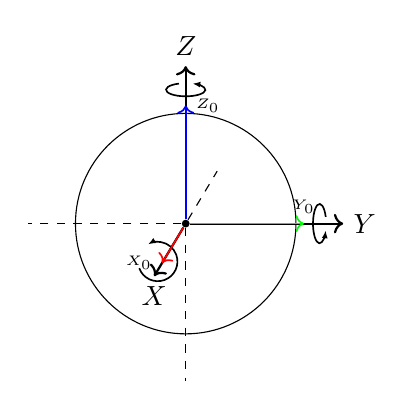
\begin{tikzpicture}
% Define radius
\def\r{2}

\draw (0,0) node[circle, fill, inner sep=1] (orig) {};
%% Bloch vector
%\draw (0, 0) node[circle, fill, inner sep=1] (orig) {} -- (\r/3, \r/2) node[circle, fill, inner sep=0.7, label=above:$\vec{a}$] (a) {};
%\draw[dashed] (orig) -- (\r/3, -\r/5) node (phi) {} -- (a);

% Sphere
\draw (orig) circle (0.7*\r);

% rotation
\draw (0, 0.85*\r) node[] (z-rot-node) {};
\draw (0.85*\r, 0) node[] (y-rot-node) {};
\draw (-0.85*\r/5, -0.85*\r/3) node[] (x-rot-node) {};

\draw[-{Latex[length=1mm]}, semithick] 
    ($(z-rot-node.center) + ({-\r*cos(70)/8}, {\r*sin(70)/24})$) 
    arc
[
    start angle=110,
    end angle=430,
    x radius=\r/8,
    y radius =\r/24
];
\draw[-{Latex[length=1mm]}, semithick] 
    ($(y-rot-node.center) + ({\r*sin(70)/24}, {\r*cos(70)/8})$) 
    arc
[
    start angle=20,
    end angle=340,
    x radius=\r/24,
    y radius =\r/8
];
\draw[-{Latex[length=1mm]}, semithick] 
    ($(x-rot-node.center) + ({-\r/8}, {0})$) 
    arc
[
    start angle=200,
    end angle=480,
    x radius=\r/8,
    y radius =\r/8
];
% Axes
\draw[dashed] (orig) -- ++(\r/5, \r/3);
\draw[dashed] (orig) -- ++(-\r, 0);
\draw[dashed] (orig) -- ++(0, -\r);
    
\draw[->, thick] (orig) -- ++(-\r/5, -\r/3) node[below] (x1) {$X$};
\draw[->, thick] (orig) -- ++(\r, 0) node[right] (x2) {$Y$};
\draw[->, thick] (orig) -- ++(0, \r) node[above] (x3) {$Z$};
    
\draw[->, semithick, red] (orig) -- ++(-0.75*\r/5, -0.75*\r/3) node[left] (x0) {\tiny \color{black}$X_0$};
\draw[->, semithick, green] (orig) -- ++(0.75*\r, 0) node[above] (y0)           {\tiny \color{black}$Y_0$};
\draw[->, semithick, blue] (orig) -- ++(0, 0.75*\r) node[right] (z0)            {\tiny \color{black}$Z_0$};
\end{tikzpicture}
        \captionof{figure}{
            Bloch sphere of qubit. 
            Each rotation arrow at the end of the axis indicates 
            RX, RY, RZ rotation.}
        \label{fig:bloch-sphere-example}
    \end{center}

    In Bloch sphere representation, Hadamard gate is a $\pi$ rotation along, $\frac{1}{\sqrt{2}}(1, 0, 1)$,
    and S gate is a $\pi/2$ rotation along, $Z$ axis.
    \begin{center}
        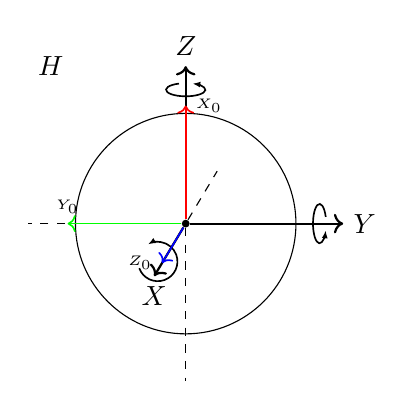
\begin{tikzpicture}
% Define radius
\def\r{2}

\draw (0,0) node[circle, fill, inner sep=1] (orig) {};
%% Bloch vector
%\draw (0, 0) node[circle, fill, inner sep=1] (orig) {} -- (\r/3, \r/2) node[circle, fill, inner sep=0.7, label=above:$\vec{a}$] (a) {};
%\draw[dashed] (orig) -- (\r/3, -\r/5) node (phi) {} -- (a);

% Sphere
\draw (orig) circle (0.7*\r);

% rotation
\draw (0, 0.85*\r) node[] (z-rot-node) {};
\draw (0.85*\r, 0) node[] (y-rot-node) {};
\draw (-0.85*\r/5, -0.85*\r/3) node[] (x-rot-node) {};

\draw[-{Latex[length=1mm]}, semithick] 
    ($(z-rot-node.center) + ({-\r*cos(70)/8}, {\r*sin(70)/24})$) 
    arc
[
    start angle=110,
    end angle=430,
    x radius=\r/8,
    y radius =\r/24
];
\draw[-{Latex[length=1mm]}, semithick] 
    ($(y-rot-node.center) + ({\r*sin(70)/24}, {\r*cos(70)/8})$) 
    arc
[
    start angle=20,
    end angle=340,
    x radius=\r/24,
    y radius =\r/8
];
\draw[-{Latex[length=1mm]}, semithick] 
    ($(x-rot-node.center) + ({-\r/8}, {0})$) 
    arc
[
    start angle=200,
    end angle=480,
    x radius=\r/8,
    y radius =\r/8
];
% Axes
\draw[dashed] (orig) -- ++(\r/5, \r/3);
\draw[dashed] (orig) -- ++(-\r, 0);
\draw[dashed] (orig) -- ++(0, -\r);
    
\draw[->, thick] (orig) -- ++(-\r/5, -\r/3) node[below] (x1) {$X$};
\draw[->, thick] (orig) -- ++(\r, 0) node[right] (x2) {$Y$};
\draw[->, thick] (orig) -- ++(0, \r) node[above] (x3) {$Z$};
    
\draw[->, semithick, red]   (orig) -- ++(0, 0.75*\r)    node[right] (x0) {\tiny \color{black}$X_0$};
\draw[->, semithick, green] (orig) -- ++(-0.75*\r, 0)                node[above] (y0)           {\tiny \color{black}$Y_0$};
\draw[->, semithick, blue]  (orig) -- ++(-0.75*\r/5, -0.75*\r/3)               node[left] (z0)            {\tiny \color{black}$Z_0$};

\draw (-\r, \r) node[right] {$H$};
\end{tikzpicture}
        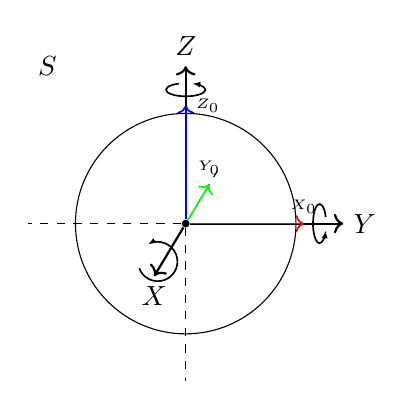
\begin{tikzpicture}
% Define radius
\def\r{2}

\draw (0,0) node[circle, fill, inner sep=1] (orig) {};
%% Bloch vector
%\draw (0, 0) node[circle, fill, inner sep=1] (orig) {} -- (\r/3, \r/2) node[circle, fill, inner sep=0.7, label=above:$\vec{a}$] (a) {};
%\draw[dashed] (orig) -- (\r/3, -\r/5) node (phi) {} -- (a);

% Sphere
\draw (orig) circle (0.7*\r);

% rotation
\draw (0, 0.85*\r) node[] (z-rot-node) {};
\draw (0.85*\r, 0) node[] (y-rot-node) {};
\draw (-0.85*\r/5, -0.85*\r/3) node[] (x-rot-node) {};

\draw[-{Latex[length=1mm]}, semithick] 
    ($(z-rot-node.center) + ({-\r*cos(70)/8}, {\r*sin(70)/24})$) 
    arc
[
    start angle=110,
    end angle=430,
    x radius=\r/8,
    y radius =\r/24
];
\draw[-{Latex[length=1mm]}, semithick] 
    ($(y-rot-node.center) + ({\r*sin(70)/24}, {\r*cos(70)/8})$) 
    arc
[
    start angle=20,
    end angle=340,
    x radius=\r/24,
    y radius =\r/8
];
\draw[-{Latex[length=1mm]}, semithick] 
    ($(x-rot-node.center) + ({-\r/8}, {0})$) 
    arc
[
    start angle=200,
    end angle=480,
    x radius=\r/8,
    y radius =\r/8
];
% Axes
\draw[dashed] (orig) -- ++(\r/5, \r/3);
\draw[dashed] (orig) -- ++(-\r, 0);
\draw[dashed] (orig) -- ++(0, -\r);
    
\draw[->, thick] (orig) -- ++(-\r/5, -\r/3) node[below] (x1) {$X$};
\draw[->, thick] (orig) -- ++(\r, 0) node[right] (x2) {$Y$};
\draw[->, thick] (orig) -- ++(0, \r) node[above] (x3) {$Z$};
    
\draw[->, semithick, red] (orig) -- ++(0.75*\r, 0) node[above] (x0) {\tiny \color{black}$X_0$};
\draw[->, semithick, green] (orig) -- ++(0.75*\r/5, 0.75*\r/3) node[above] (y0)           {\tiny \color{black}$Y_0$};
\draw[->, semithick, blue] (orig) -- ++(0, 0.75*\r) node[right] (z0)            {\tiny \color{black}$Z_0$};

\draw (-\r, \r) node[right] {$S$};
\end{tikzpicture}
        \captionof{figure}{
            Applied axis transformation by Hadamard and S gates.
            The left is a Hadamard transformation and the right is a S gate transformation.}
        \label{fig:h-s-rotation}
    \end{center}
\end{example}


\subsection{N-qubit system}

%The $\Delta t$ and norm of the Hamiltonian, $|\mathcal{H}|$ act as a rotation angle, 
%and the direction of the $\mathcal{H} \cdot \mathbf{\hat{\sigma}}$ vector acts as a rotation axis 
%on phase space of the qubit system. We will see details in the next section.
%
%A Pauli-basis of 
%$n$-qubit system 
%
%Most of the properties of Pauli-matrices are preserved in 
%$n$-fold Pauli-basis.

In the previous section, we briefly discussed basic theorems for approximating the evolution 
process with local terms, and provided a practical example with a single qubit. 
Now, we extend the construction to N-qubit systems. 
Achieving a higher-dimensional version of the operator is not possible 
by simply repeating the single-qubit operator across the entire system\footnote{Hadamard is possible, but very special case.}. 
Sometimes we only have approximation representation in higher case.
Luckily, evolution circuit is not. 
We can construct a solid structure of the circuit for multi-qubit systems,
so that we can find an exact $N$ qubit circuit 
for multi-qubit Pauli operators\footnote{We don't have to consider Solovay-Kitaev process.}.

\subsubsection{Multi qubit Pauli matrices}

\textit{Pauli strings}: Pauli string is a representation of multi-qubit Pauli operator with combination of single Pauli operators, $I, X, Y, Z$.
For example, Pauli string of $P = I \otimes X \otimes Y \otimes X$ is $IXYX$.
\index{Pauli string}
We usually called $n$-fold Pauli string when we want to emphasize the dimension.

In the previous exercise, we stated that 
the evolution on single Pauli term is same with the rotation 
along a specific axis in Hilbert-space, corresponding to the Pauli terms, $I, X, Y, Z$.
Same statement hold for $n$ qubit wires, since tensor product of Pauli terms also hold
same properties of single terms\footnote{That is why they are called by Pauli string.}.
Therefore, we can use same formula here, $R(\theta; P_i) = \cos(\theta) I+ i \sin(\theta)P_i$.


\subsubsection{Evolution as conditional rotation}

Recall the $RZ$ gate as matrix form, 

\begin{equation}
    Z = \begin{bmatrix}1 & 0 \\ 0 & -1 \end{bmatrix}, \, RZ(\theta) = \begin{bmatrix} e^{-i \theta} & 0 \\ 0 & e^{i \theta} \end{bmatrix}
\end{equation}

We can interpret the gate as conditional phase rotation by the states.

\begin{equation}
    RZ(\theta) = \begin{cases}
        |0 \rangle \rightarrow e^{- i\theta} |0\rangle \\
        |1 \rangle \rightarrow e^{  i\theta} |1\rangle \\
    \end{cases}
\end{equation}

Now observe the next Pauli term. 
We can use same convention what we did in 1 qubit Pauli Hamiltonian.

\begin{equation*}
    Z_1 Z_2 = \begin{bmatrix}
        1 & 0 & 0 & 0 \\
        0 & -1 & 0 & 0\\
        0 & 0  & -1 & 0\\
        0 & 0 & 0 & 1 
    \end{bmatrix},
    %I_1 Z_2  = \begin{bmatrix}
    %    1 & 0 & 0 & 0 \\
    %    0 & 1 & 0 & 0\\
    %    0 & 0  & -1 & 0\\
    %    0 & 0 & 0 & -1 
    %\end{bmatrix}
\end{equation*}

\begin{equation}
    \label{eq:Z1Z2_rot}
    \exp(- i \theta Z_1 Z_2) = \begin{cases}
        |\psi \rangle \rightarrow e^{- i\theta} |\psi\rangle & \mbox{if } \psi = 00 \mbox{ or } 11\\
        |\psi \rangle \rightarrow e^{  i\theta} |\psi\rangle & \mbox{if } \psi = 01 \mbox{ or } 10\\
    \end{cases}
\end{equation}

See Fig \ref{fig:evol_cir_z1z2}. It is a corresponding evolution circuit of $Z_1Z_2$ Hamiltonian. 
\begin{marginfigure}
    \centering
    \begin{quantikz}
        &\ctrl{1}& & \ctrl{1}&\\
        & \targ{}& \gate{RZ(2 \Delta t)}& \targ{} &\\
    \end{quantikz}
    \caption{Evolution circuit example of $Z_1Z_2$.}
    \label{fig:evol_cir_z1z2}
\end{marginfigure}

\subsubsection{CNOT gate}

How the CNOT gate and Rotation Z gate could implement $\exp(-i t Z_1 Z_2)$
operation? First, look at definition of CNOT gate, it flips the target 
qubit along X axis, by the control qubit state. 

\begin{center}
    \begin{quantikz}
        &\ctrl{1}&\\
        & \targ{}  &\\
    \end{quantikz} = 
    $\begin{bmatrix}
        1 & 0 & 0 & 0 \\
        0 & 1 & 0 & 0 \\
        0 & 0 & 0 & 1 \\
        0 & 0 & 1 & 0 \\
    \end{bmatrix} = (|0 \rangle \langle 0| \otimes I + |1\rangle \langle 1| \otimes X)$
    \captionof{figure}{CNOT gate}
\end{center}

Meanwhile, in basis view point, we can treat them as 
a mapping operator as 
$\{|00\rangle, |11\rangle\} \rightarrow |0\rangle$, and 
$\{|01\rangle, |10\rangle\} \rightarrow |1\rangle$.
See Fig \ref{fig:CNOT_basis}.

\begin{equation*}
    | x_1 \rangle \otimes |x_2 \rangle \rightarrow | x_1 \rangle \otimes | x_1 \oplus x_2 \rangle 
\end{equation*}

\begin{marginfigure}
    \centering
    \begin{quantikz}
        \lstick{$|{x_1}\rangle$}&\ctrl{1}&\rstick{$|x_1 \rangle$}\\
        \lstick{$|{x_2}\rangle$}&\targ{ }&\rstick{$|x_1 \oplus x_2 \rangle$}
    \end{quantikz} 
    \caption{CNOT as basis change operator.}
    \label{fig:CNOT_basis}
\end{marginfigure}

Therefore, the $I \otimes RZ(2 \Delta t)$ works of $\exp(-i \Delta t Z_1 Z_2)$ in Eq (\ref{eq:Z1Z2_rot}).

\begin{exercise}
    Is 
    \begin{quantikz}
        &\targ{}&  \gate{RZ(2 \Delta t)} & \targ{}&\\
        & \ctrl{-1}& & \ctrl{-1} &\\
    \end{quantikz} circuit identical to Fig \ref{fig:evol_cir_z1z2}? Why?
\end{exercise}

%Here we introduce the good framework to analysis the axis of the wires in each 
% Bloch sphere representation.

%\begin{example}
%    Lamor-precession of single particle in uniform magnetic field, $B$ can be formulated as next,
%
%    \begin{equation}
%        H = \mathbf{\mu} \mathbf{B}
%    \end{equation}
%\end{example}

\subsubsection{CX structure}%--------------------

\begin{figure}[!ht]
    \centering
    \begin{quantikz}
        &\ctrl{3}&           &          &                       &         &        & \ctrl{3}&\\
        &        &\ctrl{2}   &          &                       &         &\ctrl{2}&         &\\
        &        &           & \ctrl{1} &                       &\ctrl{1} &        &         &\\
        &\targ{} &\targ{}    & \targ{}  &\gate{RZ(2 \Delta t)}&\targ{}  &\targ{} &\targ{}  & 
    \end{quantikz}
    \caption{$\Delta t$ evolution circuit of $H=ZZZZ$ Hamiltonian.}
    \label{fig:ZZZ_evolve_1}
\end{figure}


In other manuscripts, next type circuit is also common.

\begin{figure}[!ht]
    \centering
    \begin{quantikz}
        &\ctrl{1}&           &          &                     &         &        &\ctrl{1}&\\
        &\targ{} &\ctrl{1}   &          &                     &         &\ctrl{1}&\targ{} &\\
        &        &\targ{}    & \ctrl{1} &                     &\ctrl{1} &\targ{} &        &\\
        &        &           & \targ{} &\gate{RZ(2 \Delta t)} &\targ{}  &        &        &
    \end{quantikz}
    \caption{$\Delta t$ evolution circuit of $H=ZZZZ$ Hamiltonian 2nd type.}
    \label{fig:ZZZ_evolve_2}
\end{figure}

The Fig \ref{fig:ZZZ_evolve_1} is called by \textit{fountain} type, 
and Fig \ref{fig:ZZZ_evolve_2} is called by \textit{chain} type.

\begin{exercise}
    Show that the above two circuits are identical. 
    Do not use a matrix representation. \textit{Hint: See a property of direct sum or bitwise XOR, both are identical in binary vector}.
\end{exercise}

If you construct the circuit in matrix form,
you can verify that those two circuits are identical.
In the end, the mixture of two type also identical
and the position of the $RZ$ gate is also freely determined
by the situation. 
The only thing we need is a CNOT gate path
visit each i-th qubits in the Hamiltonian at once\footnote{Considering qubit rearangement.}.

\begin{center}
\begin{quantikz}
    &\ctrl{3}&           &          &                      &             &           &\ctrl{3}&\\
    &        &\targ{}    & \targ{}  & \gate{RZ(2 \Delta t)}& \targ{}     & \targ{}   &       &\\
    &        &           & \ctrl{-1}&                      & \ctrl{-1}   &           &       &\\
    &\targ{} &\ctrl{-2}  &          &                      &             & \ctrl{-2} &\targ{}&
\end{quantikz}
\end{center}

\subsubsection{Basis transformation}

We only analyzed $I, Z$ strings. 
General strings consist of $I, Z, X, Y$ yields next circuit for evolution operator.


\begin{equation}
    \exp(-i \Delta t XYZZ)
\end{equation}

\begin{figure}[!ht]
    \centering
    \begin{quantikz}
       &\gate{H}         &          &\ctrl{1}&           &          &                     &         &        &\ctrl{1}& \gate{H}&         &\\
       &\gate{S^\dagger} & \gate{H} &\targ{} &\ctrl{1}   &          &                     &         &\ctrl{1}&\targ{} & \gate{H}& \gate{S}&\\
       &                 &          &        &\targ{}    & \ctrl{1} &                     &\ctrl{1} &\targ{} &        &         &         & \\
       &                 &          &        &           & \targ{} &\gate{RZ(2 \Delta t)} &\targ{}  &        &        &         &         & 
    \end{quantikz}
\end{figure}

\begin{example}
    Understanding the circuit with graphic notation of basis.

\end{example}


\subsection{Implementation with Phase operator}

The evolution circuit was a conditional phase rotation by 
the system state. There is a Phase operator in quantum 
computer.

\begin{equation*}
    \mbox{P}(\theta) = \begin{bmatrix}
        1 & 0 \\
        0 & e^{i \theta}
    \end{bmatrix}, 
    \mbox{RZ}(\theta) = \begin{bmatrix}
        e^{-i \theta/2} & 0 \\
        0 & e^{i \theta/2}
    \end{bmatrix}
\end{equation*}

\begin{marginfigure}
    \begin{quantikz}
        &\ctrl{1}&\\
        &\gate{P(\theta)}&
    \end{quantikz}
\end{marginfigure}

They are same in single qubit system, however, in multi-qubit system a rotation z gate and 
a phase gate work differently because of the local phases.
Even though, we can implement the same operation
with phase gates without rotation z gates.

\begin{center}
    \begin{quantikz}
        & \ctrl{1} &                  & \ctrl{1} & \\
        & \targ{}  & \gate{RZ(\theta)} & \targ{} &
    \end{quantikz}
    = $e^{-i \theta/2} \begin{bmatrix}
    1 & 0 & 0 & 0 \\
    0 & e^{i \theta} & 0 &0\\
    0 & 0 & e^{i \theta}& 0\\
    0 & 0 & 0   & 1
    \end{bmatrix}$
    \\
    \begin{quantikz}
        & \gate{P(\alpha)} & \ctrl{1} & \\
        & \gate{P(\beta)}  & \gate{P(\gamma)} &
    \end{quantikz}
    = $\begin{bmatrix}
    1 & 0 & 0 & 0 \\
    0 & e^{i \beta} & 0 &0\\
    0 & 0 & e^{i \alpha}& 0\\
    0 & 0 & 0   & e^{i (\alpha + \beta) \gamma} 
    \end{bmatrix}$
\end{center}

If $\alpha = \beta = \theta$ and $\gamma = -2 \theta$, the two circuit are identical
without considering global phase.
Similarly, we can arange RZ gates to construct the evolution circuit 
without CX gate, but using controlled-RZ gate.

\begin{exercise}
    Show that the RZ and controlled-RZ could generate $ZZ, IZ, ZI$ evolution gate 
    on 2 qubit circuit. 
\end{exercise}


Note that, when you work with gate model,
it is very common case that using an ancilla registers
to reduce the circuit depth, or to implement some algorithms.
During the process, you must take care of the relative 
phase between the original register and the ancilla register.
Sometimes it does not affect but before the calculation 
you must ensure the consistency.
Think about Ahrno-Bohm effect, it is not a strange 
effect that the local phase difference affect the overall
result.


\section{Additional Note}


\subsection{Clifford Group}

The evolution circuit comprise large 3 gate sets.

\begin{itemize}
    \item Rotation gates: $RZ$
    \item Entaglement gates: $CNOT$
    \item Basis Transformation gates: $H, S$
\end{itemize}


For example, using two rotation gates, $RZ, RX$
we can eliminate $H, S$ gates in the evolution circuit.
On the other hand, we can use 3 rotation gates
without those basis change gates. 


% 2 qubit gates

% 3 -qubit gates



\subsection{Pauli-Frame}

As a rotation, geographical representation only work for 
1-qubit case.
In $N$-qubit case, there is no representation method 
including all quantum information and state.
Same hold for each rotation gate in Trotterization circuit.
We accept the circuit in Fig () is a rotation around axis \textbf{nemo}.
What about the next figure?


Back to the conditional rotation interpretation of 
the evolution matrix.



There is an additional physical meaning in Pauli Frame.
It represents a mutually commuting axes set that we 
can manipulate on the circuit.

%======================================================================================================================================

\newpage
\chapter{Optimization of evolution circuit}
\section{Introduction}

The optimization of quantum circuit has various meaning by the contenxt. 
In this section, the term \textit{optimization} is used as indicating two concept.
First is error reducing technique of circuit representation of time-evolution dynamics, 
and Second is a direct circuit depth reduction techniques.

\section{Mutally commuting groups}

In the Product formula, Eq(\ref{eq:product_formula}), 
the total time evolution operator is approximated with product of several local Hamiltonian operators.
It is just an approximation but actively adopted in many references and methods. % Trotter formula reference 와 QAOA 방법론 언급
The reason is that we don't know proper method to find exact evolution operator corresponding to the total Hamiltonian.
Moreover, the method represents the locality of the given system well. % cite trotter error paper.
In such representation, the product order of local operators does not affect the \textit{physical} system or 
ther is no dependence on the system.
It is purely error reduction technique of the implementation.

Start from the 3 terms, $A, B, C$ hermite operators, 
the given Hamiltonian is $H = A +  B +  C$.
By the BCH formula, the product of $\exp(A) \exp(B) \exp(C)$ has next error terms.

\begin{eqnarray}
    \exp(A)\exp(B) &=& \exp(A+B) \exp(\Theta(A, B))\\
    \exp(A + B)\exp(C) &=& \exp(A + B + C) \exp(\Theta((A+ B), C))\\
    \exp(A)\exp(B)\exp(C) &=& \exp(A+B+C) \exp(\Theta((A+B), C) - \Theta(A, B)) 
\end{eqnarray}

However, the error term $\Theta(A, B) = \Theta([A, B])$ and $\Theta(0) = 0$,
it means that in the case of commuting operators $[A, B] = [B, C] = [A, C] = 0$, 
the product formula is exactly same the proper time evolution operator,

\begin{equation}
    \exp(A)\exp(B)\exp(C) = \exp(A + B + C)
\end{equation}

It is not a general case of the simulation, however, there are mutually commuting subsets exists generally.
The situation of every local Hamitlonians are anti-commuting each other is also a rare case as much as the all commuting case.

Childs et al derived product formula error with commutator scaling\cite{PhysRevX.11.011020}.

\begin{theorem}\textbf{Product error with commutator scaling}
    
    Let, $\mathcal{L}_p(H, t)$ be a $p$-th order product formula of the given Hamiltonian, $H = \sum_i H_i$.
    Then, the error of the $p$-th order approximation is 

    \begin{equation}
        \| \mathcal{L}_p(H ,t) - \exp(-i t H) \| = \mathcal{O}(\tilde{\alpha}_{com} t^{p+1}),
    \end{equation}
    where, $\tilde{\alpha}_{com} := \sum_{\lambda_1, \lambda_2, \dots , \lambda_{p+1}} \Vert[H_{\lambda_{p+1}}, \dots [H_{\lambda_2}, H_{\lambda_1}]] \Vert$
    
\end{theorem}

The reduction of big-O error does not significantly large, however, mutually commuting group allow us some freedom to manipulate additional optimization about the circuit gates.

\section{Hamiltonian grouping problem}

We can construct a graph of which edges are indicating commuting, anti-commuting relathion of Pauli nodes.
Such graph is called \textit{compatible graph}. 
Fig (\ref{fig:compatible_graph_example}) is a example compatible graph of 1 qubit system.

\begin{center}
    \centering
    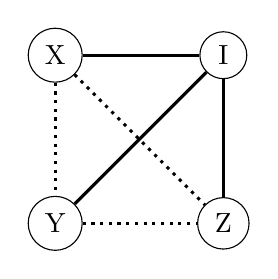
\begin{tikzpicture}
        \node[regular polygon, regular polygon sides=4, minimum size=3cm] at (0,0) (A) {};
        \node[circle, fill=white, draw=black] (I) at (A.corner 1) {I};
        \node[circle, fill=white, draw=black] (X) at (A.corner 2) {X};
        \node[circle, fill=white, draw=black] (Y) at (A.corner 3) {Y};
        \node[circle, fill=white, draw=black] (Z) at (A.corner 4) {Z};
        
        \draw[line width=0.4mm, black ,-] (I) -- (X) ;
        \draw[line width=0.4mm, black ,-] (I) -- (Y) ;
        \draw[line width=0.4mm, black ,-] (I) -- (Z) ;

        \draw[line width=0.4mm, black , dotted] (X) -- (Y) ;
        \draw[line width=0.4mm, black , dotted] (X) -- (Z) ;
        \draw[line width=0.4mm, black , dotted] (Y) -- (Z) ;
    \end{tikzpicture}
    \captionof{figure}{The straight line indicates commuting relationship of two ends of the edge and 
    the dottted line indicates anti-commuting relathinship.}
    \label{fig:compatible_graph_example}
\end{center}
The $n$-qubit system also has such compatible graph of 
$n$-fold Pauli-strings. It is beacuse the $n$ fold Pauli string 
always either anti-commute or commute each other.
\begin{equation}
    [P_i^n, P_j^n] =0 \, \mbox{or} \, \{P_i^n, P_j^n\} =0
\end{equation}
where, $[]$ is a commutator and $\{\}$ is an anti-commutator.
Since, any given Hamiltonian has a $n$-folded Pauli-polynomial represenation, 
a specific Hamiltonian would be represented as a subgraph, $G_{\mathcal{H}}$ of nodes in 
the $n$-fold compatible graph, $G$.

We can reduce a commuting error 
by minimizing the number of nested pair of anti-commuting 
Pauli-strings on the circuit. 
It is equivalent to finding a mutually commuting partition
of Pauli-set.

\begin{definition}{\textbf{Pauli Partitioning Problem}}

    For a set of $n$ fold Pauli strings, $\mathcal{P}^\ast$,
    and a given subcollection $\mathbf{S} \subseteq \mathcal{P}^\ast$, 
    Pauli Partitioning Problem(PPP) is to return a partition of $\mathbf{S}$ into the fewest number of commuting parts.
\end{definition}

%Constructing a collection $\mathcal{M}_c$ st that for all $C \in \mathcal{M}_c$, 
\begin{equation}
    [p_i, p_j] =0 \, \forall p_i, p_j \in P_l \in \mathbf{S}
\end{equation}

where, $\forall p_i$ is a pauli-string. 

However, determining the commutation of the arbitary Pauli-strings 
and find a mutually commuting partition both of are not simple jobs.

are conceptually easy but computationally, it is a tedious work.

\subsection{Commutator of n-folded string}

There are two common method to determine the commutation relationship of $n$ folded Pauli-strings.
\textit{general commutativity}, and \textit{qubit-wise-commutativity}\cite{gokhale_on3_2020}. % citation

\begin{theorem}\textbf{General-Commutattivity}(GC)

    For $n$-folded Pauli string, $P_j^n = \otimes_i^n p_i^j, P_k^n = \otimes_i^n p_i^k$,
    
    \begin{equation}
        [P_j^n, P_k^n] = 0 \Leftrightarrow \forall i, \mbox{occurence of } \{p_i^j, p_i^k\} = 0 \mbox{ is } 2l,\, l \in \mathbb{Z}_+ 
    \end{equation}
\end{theorem}

\begin{theorem}\textbf{Qubit-Wise-Commutattivity}(QWC)

    For $n$-folded Pauli string, $P_j^n = \otimes_i^n p_i^j, P_k^n = \otimes_i^n p_i^k$,
    \begin{equation}
        \forall i, \{p_i^j, p_i^k\} = 0 \Rightarrow [P_j^n, P_k^n] = 0
    \end{equation}
\end{theorem}

QWC is a sub-relationship of GC. QWC commuting or anti-commuting pair is a commuting or anti-commuting pair in GC.
A reverse is not hold in general case.


The problem is for $n$-qubits system, there are $2^n$ number of Pauli-strings.
Constructing commuting/anti-commuting map of the Pauli-strings requires next number of operations with GC.

\begin{equation}
    \left( \begin{matrix} 2^n \\ 2 \end{matrix} \right) n = O(4^n n)
\end{equation}

It has an expotential time complexity to achieve the compatible graph. 
Therefore, some frameworks only offer QWC method or providing 
pre-calculated commuting set in restricted dimension. % Pennylane 예시 넣고 IBM Qiskit도 찾아보기


Reggio et al suggested acceleration technique in commuting term determinantion
\cite{reggio_fast_2023}. 
The similar result was introduced in 2009 from theories of Möbius pair of simplices by Havlicek et al\cite{havlicek_moebius_2009}.
They decompose the Pauli-term into two faimilies and represent the strings as product of two family memebers.
For example, $X, Z$ families are

\begin{itemize}
    \item $X$-family: $IIIX$, $XIXI$, $IIXI$, $IXXX, \dots$
    \item $Z$-family: $IIIZ$, $ZIZI$, $IIZI$, $IZZZ, \dots$
\end{itemize}
then, every Pauli string, even a string containing $Y$ elements, can be represented 
with a production of two families, $x_i \cdot z_j$.
For example, 
\begin{equation}
    P_l = YZIX = (XIIX) \cdot (ZZII) = x_i \cdot z_j
\end{equation}

\begin{theorem}
    
    For a given pair of two $n$-fold Pauli strings, $P_i, P_j$,
    there is a X, Z family product representation as 

    \begin{itemize}
        \item $P_i = x_k \cdot z_l$
        \item $P_j = x_m \cdot z_n$
    \end{itemize}.

    then the given pair strings are commuting each other if and only if 
    $[z_l, x_m] =  [z_n, x_k]$.

\end{theorem}

Simply,

\begin{equation}
    [P_i, P_j] = [x_k \cdot z_i, x_m \cdot z_n] = \begin{cases} 
        0 & \mbox{if } \, [z_i, x_m] = [x_k, z_n] \\
        -P_i P_j & \mbox{otherwise}
     \end{cases}
\end{equation}

This allows us to determine the commutation of two $n$ fold string with only a few 
operations of 4 binary values. 
Unfortunately, this method does not allow us to avoid expotential 
cost increasing for larger $n$.

\subsubsection{Sympletic representation of Pauli element}

The XZ code is a kind of sympletic representation of Pauli group 
element.

Using this notation you can represent 
the various algebra with simple integer operations,
not a $2^n \times 2^n$ dimension matrix operation.

\begin{itemize}
    \item Group addition:
    \item Linear combination:
    \item Tensor product:
\end{itemize}

In addition, the XZ code itself is a specific matrix index 
where, the each Pauli terms are mapped into standard basis of matrix space.

\begin{equation}
    P_i = e_i
\end{equation}

Using this representation, you can fastly decompose the 
given Hamiltonian as Pauli-polynomial. See details in Append \ref{appendix:FPPM}.

\subsection{Partition construction}

Once the compatible graph is constructed, the task at hand is to search for the 
mutually commuting partitions from the given compatible graph of Pauli-strigns.
It is equivalent with Max-clique problem\footnote[3]{See details of Max-clique problems in Appendix \ref{appendix:max-clique}}, 
unfortunately, it is a well known NP problem\cite{miller_reducibility_1972}.
There have been many attemptions to solve or approximate the solution of the problem.
However, in this documnet, we would like to indtroduce 
Adiabatic approximation technique suggested by Kurita et al\cite{kurital_2023}.

\begin{figure}[ht]
    \centering
    \scalebox{0.7}{
        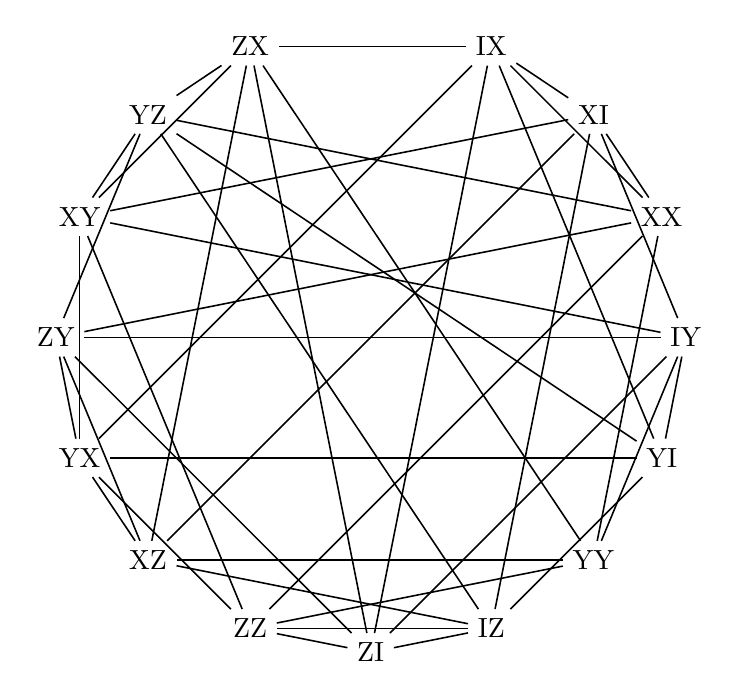
\begin{tikzpicture}
            \node[] (IX) at (2*0.7653668647301797 , 2* 1.847759065022573)    {IX};
            \node[] (XI) at (2*1.4142135623730951 , 2*1.414213562373095)    {XI};
            \node[] (XX) at (2*1.8477590650225735 , 2*0.7653668647301796)   {XX};
            \node[] (IY) at (2*2.0, 0.0)                                  {IY};
            \node[] (YI) at (2* 1.847759065022573 , 2*-0.7653668647301808)   {YI};
            \node[] (YY) at (2* 1.4142135623730947 , 2*-1.4142135623730954)  {YY};
            \node[] (IZ) at (2* 0.76536686473018 , 2*-1.8477590650225733)    {IZ};
            \node[] (ZI) at (2* 0 , 2*-2.0)                                  {ZI};
            \node[] (ZZ) at (2* -0.7653668647301807 , 2*-1.847759065022573)  {ZZ};
            \node[] (XZ) at (2* -1.4142135623730954 , 2*-1.414213562373095)  {XZ};
            \node[] (YX) at (2* -1.8477590650225737 , 2*-0.7653668647301793) {YX};
            \node[] (ZY) at (2* -2.0 , 2*0)                                  {ZY};
            \node[] (XY) at (2* -1.8477590650225735 , 2*0.7653668647301798)  {XY};
            \node[] (YZ) at (2* -1.414213562373095 , 2*1.4142135623730951)   {YZ};
            \node[] (ZX) at (2* -0.7653668647301795 , 2*1.8477590650225735)  {ZX};

            \draw[line width=0.2mm, black ,-] (IX) -- (ZX) ;
            \draw[line width=0.2mm, black ,-] (IX) -- (YX) ;
            \draw[line width=0.2mm, black ,-] (IX) -- (ZI) ;
            \draw[line width=0.2mm, black ,-] (IX) -- (YI) ;
            \draw[line width=0.2mm, black ,-] (IX) -- (XX) ;
            \draw[line width=0.2mm, black ,-] (IX) -- (XI) ;

            \draw[line width=0.2mm, black ,-] (XI) -- (XY) ;
            \draw[line width=0.2mm, black ,-] (XI) -- (XZ) ;
            \draw[line width=0.2mm, black ,-] (XI) -- (IZ) ;
            \draw[line width=0.2mm, black ,-] (XI) -- (IY) ;
            \draw[line width=0.2mm, black ,-] (XI) -- (XX) ;

            \draw[line width=0.2mm, black ,-] (XX) -- (YZ);
            \draw[line width=0.2mm, black ,-] (XX) -- (ZY);
            \draw[line width=0.2mm, black ,-] (XX) -- (ZZ);
            \draw[line width=0.2mm, black ,-] (XX) -- (YY);

            \draw[line width=0.2mm, black ,-] (IY) -- (XY);
            \draw[line width=0.2mm, black ,-] (IY) -- (ZY);
            \draw[line width=0.2mm, black ,-] (IY) -- (ZI);
            \draw[line width=0.2mm, black ,-] (IY) -- (YY);
            \draw[line width=0.2mm, black ,-] (IY) -- (YI);

            \draw[line width=0.2mm, black ,-] (YI) -- (YZ);
            \draw[line width=0.2mm, black ,-] (YI) -- (YX);
            \draw[line width=0.2mm, black ,-] (YI) -- (IZ);

            \draw[line width=0.2mm, black ,-] (YY) -- (ZX);
            \draw[line width=0.2mm, black ,-] (YY) -- (XZ);
            \draw[line width=0.2mm, black ,-] (YY) -- (ZZ);

            \draw[line width=0.2mm, black ,-] (IZ) -- (YZ);
            \draw[line width=0.2mm, black ,-] (IZ) -- (XZ);
            \draw[line width=0.2mm, black ,-] (IZ) -- (ZZ);
            \draw[line width=0.2mm, black ,-] (IZ) -- (ZI);

            \draw[line width=0.2mm, black ,-] (ZI) -- (ZX);
            \draw[line width=0.2mm, black ,-] (ZI) -- (ZY);
            \draw[line width=0.2mm, black ,-] (ZI) -- (ZZ);
            
            \draw[line width=0.2mm, black ,-] (ZZ) -- (XY);
            \draw[line width=0.2mm, black ,-] (ZZ) -- (YX);
        

            \draw[line width=0.2mm, black ,-] (XZ) -- (ZX);
            \draw[line width=0.2mm, black ,-] (XZ) -- (ZY);
            \draw[line width=0.2mm, black ,-] (XZ) -- (YX);

            \draw[line width=0.2mm, black ,-] (YX) -- (XY);
            \draw[line width=0.2mm, black ,-] (YX) -- (ZY);

            \draw[line width=0.2mm, black ,-] (ZY) -- (YZ);

            \draw[line width=0.2mm, black ,-] (XY) -- (ZX);
            \draw[line width=0.2mm, black ,-] (XY) -- (YZ);

            \draw[line width=0.2mm, black ,-] (ZX) -- (YZ);
        \end{tikzpicture}
        \begin{tikzpicture}
    \node[] (IX) at (2*0.7653668647301797 , 2* 1.847759065022573)    {IX};
    \node[] (XI) at (2*1.4142135623730951 , 2*1.414213562373095)    {XI};
    \node[] (XX) at (2*1.8477590650225735 , 2*0.7653668647301796)   {XX};
    \node[] (IY) at (2*2.0, 0.0)                                  {IY};
    \node[] (YI) at (2* 1.847759065022573 , 2*-0.7653668647301808)   {YI};
    \node[] (YY) at (2* 1.4142135623730947 , 2*-1.4142135623730954)  {YY};
    \node[] (IZ) at (2* 0.76536686473018 , 2*-1.8477590650225733)    {IZ};
    \node[] (ZI) at (2* 0 , 2*-2.0)                                  {ZI};
    \node[] (ZZ) at (2* -0.7653668647301807 , 2*-1.847759065022573)  {ZZ};
    \node[] (XZ) at (2* -1.4142135623730954 , 2*-1.414213562373095)  {XZ};
    \node[] (YX) at (2* -1.8477590650225737 , 2*-0.7653668647301793) {YX};
    \node[] (ZY) at (2* -2.0 , 2*0)                                  {ZY};
    \node[] (XY) at (2* -1.8477590650225735 , 2*0.7653668647301798)  {XY};
    \node[] (YZ) at (2* -1.414213562373095 , 2*1.4142135623730951)   {YZ};
    \node[] (ZX) at (2* -0.7653668647301795 , 2*1.8477590650225735)  {ZX};

    \draw[line width=0.2mm, green ,-] (IX) -- (XX) ;
    \draw[line width=0.2mm, green ,-] (IX) -- (XI) ;
    \draw[line width=0.2mm, green ,-] (XI) -- (XX) ;

    \draw[line width=0.2mm, green ,-] (IY) -- (YY);
    \draw[line width=0.2mm, green ,-] (IY) -- (YI);
    \draw[line width=0.2mm, green ,-] (YI) -- (YY);

    \draw[line width=0.2mm, green ,-] (IZ) -- (ZZ);
    \draw[line width=0.2mm, green ,-] (IZ) -- (ZI);
    \draw[line width=0.2mm, green ,-] (ZI) -- (ZZ);

    \draw[line width=0.2mm, green ,-] (XZ) -- (YX);
    \draw[line width=0.2mm, green ,-] (XZ) -- (ZY);
    \draw[line width=0.2mm, green ,-] (YX) -- (ZY);


    \draw[line width=0.2mm, green ,-] (XY) -- (ZX);
    \draw[line width=0.2mm, green ,-] (XY) -- (YZ);
    \draw[line width=0.2mm, green ,-] (ZX) -- (YZ);
\end{tikzpicture}
        }
    \caption{
        Left: Compatible graph of 2-qubit system Pauli-strings. 
        Each edge indicates commuting relationship between the two ends.
        The edges in the figure weighted zero, and edges between disconnected nodes
        are weighted as 1.
        Right:
        The figure was refered from Kurita et al. 2023, redrawed by the author\cite{kurital_2023}.
    }
    \label{fig:compatible_graph_example_2qubits}
\end{figure}
%\begin{figure}[ht]
%    \centering
%        \begin{tikzpicture}
    \node[] (IX) at (2*0.7653668647301797 , 2* 1.847759065022573)    {IX};
    \node[] (XI) at (2*1.4142135623730951 , 2*1.414213562373095)    {XI};
    \node[] (XX) at (2*1.8477590650225735 , 2*0.7653668647301796)   {XX};
    \node[] (IY) at (2*2.0, 0.0)                                  {IY};
    \node[] (YI) at (2* 1.847759065022573 , 2*-0.7653668647301808)   {YI};
    \node[] (YY) at (2* 1.4142135623730947 , 2*-1.4142135623730954)  {YY};
    \node[] (IZ) at (2* 0.76536686473018 , 2*-1.8477590650225733)    {IZ};
    \node[] (ZI) at (2* 0 , 2*-2.0)                                  {ZI};
    \node[] (ZZ) at (2* -0.7653668647301807 , 2*-1.847759065022573)  {ZZ};
    \node[] (XZ) at (2* -1.4142135623730954 , 2*-1.414213562373095)  {XZ};
    \node[] (YX) at (2* -1.8477590650225737 , 2*-0.7653668647301793) {YX};
    \node[] (ZY) at (2* -2.0 , 2*0)                                  {ZY};
    \node[] (XY) at (2* -1.8477590650225735 , 2*0.7653668647301798)  {XY};
    \node[] (YZ) at (2* -1.414213562373095 , 2*1.4142135623730951)   {YZ};
    \node[] (ZX) at (2* -0.7653668647301795 , 2*1.8477590650225735)  {ZX};

    \draw[line width=0.2mm, green ,-] (IX) -- (XX) ;
    \draw[line width=0.2mm, green ,-] (IX) -- (XI) ;
    \draw[line width=0.2mm, green ,-] (XI) -- (XX) ;

    \draw[line width=0.2mm, green ,-] (IY) -- (YY);
    \draw[line width=0.2mm, green ,-] (IY) -- (YI);
    \draw[line width=0.2mm, green ,-] (YI) -- (YY);

    \draw[line width=0.2mm, green ,-] (IZ) -- (ZZ);
    \draw[line width=0.2mm, green ,-] (IZ) -- (ZI);
    \draw[line width=0.2mm, green ,-] (ZI) -- (ZZ);

    \draw[line width=0.2mm, green ,-] (XZ) -- (YX);
    \draw[line width=0.2mm, green ,-] (XZ) -- (ZY);
    \draw[line width=0.2mm, green ,-] (YX) -- (ZY);


    \draw[line width=0.2mm, green ,-] (XY) -- (ZX);
    \draw[line width=0.2mm, green ,-] (XY) -- (YZ);
    \draw[line width=0.2mm, green ,-] (ZX) -- (YZ);
\end{tikzpicture}
%        \caption{
%            Example of mutually commuting partition of Fig (\ref{fig:compatible_graph_example_2qubits})
%            }
%        \label{fig:compatible_graph_example_2qubits-commuting-set}
%\end{figure}

Kurita et al used a graph partitioning Hamiltonian and 
constructed sequetial clique extracting algorithm.
The compatible graph modeled as binary, 0 and 1, weighted 
complete graph by edges of commutation are marked as 0 
and the anti-commutation ones are marked as 1.
Basic procedure of Kurita et al is 

\begin{enumerate}
    \item Extract max-clique set, $P_i$, from the compatible graph.
    \item Delete the nodes which were extracted from the step 1 from the graph.
    \item Repeat until there is no remaining node after step 2.
\end{enumerate}.

The mutually commuting partitions are constructed 
by each max-cliques, $\{P_i\}_{i=1}^N$. 
The mutually commutation relationship is guaranteed by the next 
Hamiltonian, quadratic ising model.

\begin{equation}
    \mathcal{H} = -\sum_i Z_i + \sum_{i >j} Z_i Zj
\end{equation}

The first term, $-\sum_i Z_i$, reduces the state energy 
proportional to a number of nodes in the clique.
The seocond term, $\sum_{i >j} Z_i Zj$ rasies the state energy
as much of the number of the anti-commuting terms in the sample.
At each step, the clique searching was conducted by stimulated annealing chip provided by Fujititu. 


%\section{Pauli Frame}
%
%In the evolution circuit of the specific Pauli string, the circuit consist of several manipulation terms by the configuration of the CNOT gates.
%
%Even if, there are $N'$ number of mutually commuting Pauli-strings, 
%the single operation step evolution only possible for $N$ number of the strings. 
%$N$ is a number of qubits in the algorithm.


\section{Axis transformation weight}

The main idea of Kurita et al allow us to find 
mutually commuting partition of the given 
Hamiltonian set. 
However, there are some degeneracy in extracting cliques 
from the pauli-graph of the given Hamiltonian.

Consider the next Pauli graph.

\begin{center}
    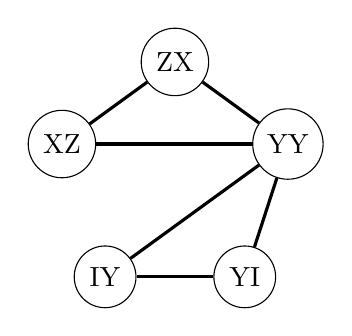
\begin{tikzpicture}
        \node[regular polygon, regular polygon sides=5, minimum size=3cm] at (0,0) (A) {};
        \node[circle, fill=white, draw=black] (zx) at (A.corner 1) {ZX};
        \node[circle, fill=white, draw=black] (xz) at (A.corner 2) {XZ};
        \node[circle, fill=white, draw=black] (iy) at (A.corner 3) {IY};
        \node[circle, fill=white, draw=black] (yi) at (A.corner 4) {YI};
        \node[circle, fill=white, draw=black] (yy) at (A.corner 5) {YY};

        \draw[line width=0.4mm, black ,-] (xz) -- (zx) ;
        \draw[line width=0.4mm, black ,-] (xz) -- (yy) ;
        \draw[line width=0.4mm, black ,-] (zx) -- (yy) ;
        \draw[line width=0.4mm, black ,-] (yy) -- (iy) ;
        \draw[line width=0.4mm, black ,-] (yy) -- (yi) ;
        \draw[line width=0.4mm, black ,-] (iy) -- (yi) ;
        %\foreach \i[evaluate={\j=int(17-\i)}] in {2,...,15}
        %    \node[circle, fill=white, draw=black, ultra thick] (\j) at (A.corner \i) {$B_{\j}$};
        % Line
        %\foreach \i[evaluate={\j=int(int(\i+1) - int((\i+1)/16))}] in {0, ..., 15}
        %    \draw[line width=0.1mm, black ,-] (\i) -- (\j);
    \end{tikzpicture}
\end{center}

We have two possible partitions in the optimization process.

\begin{center}
    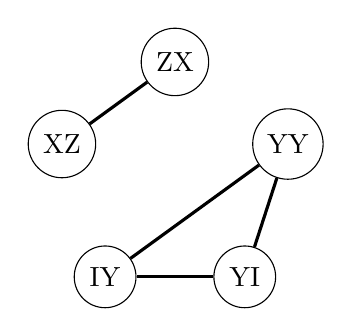
\begin{tikzpicture}
        \node[regular polygon, regular polygon sides=5, minimum size=3cm] at (0,0) (A) {};
        \node[circle, fill=white, draw=black] (zx) at (A.corner 1) {ZX};
        \node[circle, fill=white, draw=black] (xz) at (A.corner 2) {XZ};
        \node[circle, fill=white, draw=black] (iy) at (A.corner 3) {IY};
        \node[circle, fill=white, draw=black] (yi) at (A.corner 4) {YI};
        \node[circle, fill=white, draw=black] (yy) at (A.corner 5) {YY};

        \draw[line width=0.4mm, black ,-] (xz) -- (zx) ;
        \draw[line width=0.4mm, black ,-] (yy) -- (iy) ;
        \draw[line width=0.4mm, black ,-] (yy) -- (yi) ;
        \draw[line width=0.4mm, black ,-] (iy) -- (yi) ;
    \end{tikzpicture}
    \hspace{1cm}
    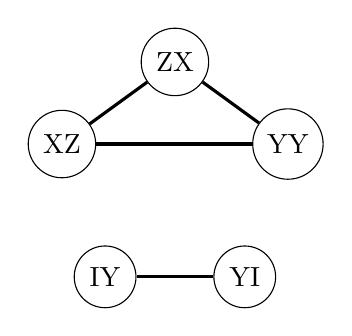
\begin{tikzpicture}
        \node[regular polygon, regular polygon sides=5, minimum size=3cm] at (0,0) (A) {};
        \node[circle, fill=white, draw=black] (zx) at (A.corner 1) {ZX};
        \node[circle, fill=white, draw=black] (xz) at (A.corner 2) {XZ};
        \node[circle, fill=white, draw=black] (iy) at (A.corner 3) {IY};
        \node[circle, fill=white, draw=black] (yi) at (A.corner 4) {YI};
        \node[circle, fill=white, draw=black] (yy) at (A.corner 5) {YY};

        \draw[line width=0.4mm, black ,-] (xz) -- (zx) ;
        \draw[line width=0.4mm, black ,-] (xz) -- (yy) ;
        \draw[line width=0.4mm, black ,-] (zx) -- (yy) ;
        \draw[line width=0.4mm, black ,-] (iy) -- (yi) ;
    \end{tikzpicture}
\end{center}

These two partition are indistinguishable in binary weighted 
graph suggested by Kurita et al. 
That means, the system has a degeneracy in the ground state.
In general, each intermediate steps we would face such degeneracy 
in the max-clique finding problem.
However, if we consider an additional implementation cost 
on the circuit, we can remove such degeneracy from the process.
The author, Kim, suggested basis transformation weight to the 
Kurita's Hamiltonian.

In 2 qubit system, general evolution operator of length two Pauli-string on circuit would
have next form.

\begin{center}
\begin{quantikz}
    & \gate{B_1} & \ctrl{1}& & \ctrl{1} & \gate{B_1^\dagger}\\
    & \gate{B_2} & \targ{} & \gate{RZ(2\Delta t)}& \targ{} & \gate{B_2^\dagger}\\
\end{quantikz}
\end{center}

By the axis of the rotation, 
the basis transformation gates rotate the qubit axes.
However, some cases intermediate gates between 
rotation gates are not necessary to exist.
If the nested rotation axes, mutually commuting 
by the method of implementation we can ignore the basis transformation circuit.
See an example and details in \textit{Pauli-Frame}.

Two parameters could be considered in the problem.

\begin{itemize}
    \item Circuit depth
    \item Number of gates 
\end{itemize}

\subsection{Rough implementation of single qubit transformation}

Transformation method to the graph clique problem and
corresponding problem is well established in Kurita et al.

\begin{center}
    \begin{quantikz}
        & \gate{B} &
    \end{quantikz}
     = \begin{quantikz}
         \gate{H} 
    \end{quantikz} or \begin{quantikz}
         \gate{S^\dagger} & \gate{H}
    \end{quantikz}
\end{center}

\begin{definition}{\textbf{Single qubit transformation depth}}
    
    The transformation depth of the nested axes, $A_1, A_2$ is defined as,
    \begin{equation}
        w(\cdot) : P^1 \times P^1 \rightarrow \mathbb{Z}_+
    \end{equation}

    where, $P^1 = \{I, X, Y, Z\}$.
\end{definition}

\begin{center}
    \begin{tabular}{c c c}
        \hline
        Nested Axes & Transformation gate & Transformation Depth\\
        \hline
        A A & $I    $ & 0 \\
        Z X & $H    $ & 1 \\
        Z Y & $S^\dagger H  $  & 2 \\
        X Y & $H S^\dagger H$ & 3\\
    \end{tabular}
\end{center}

Expand them to the multi-qubit Hamiltonian, then 

\begin{equation}
    W(S_i, S_j) := \frac{1}{N} \sum_{k=1}^N w((S_i)_k, (S_j)_k) 
\end{equation}


\begin{equation}
    \mathcal{H} = - \mu_o \sum  Z_i + \mu_1 \sum_{i <j} h_{ij} Z_iZ_j + \mu_2 \sum_{i<j} w_{ij} Z_i Z_j
\end{equation}

where, $h_{ij} \in \{0, 1\}$ and $w_{ij} \in [0, 1]$.

To avoid the reversed energy of the commuting and non-commuting 
states, the prior coefficients, $\mu_0, \mu_1, \mu_2$ must satisfies the next constraints,

\begin{equation}
    \begin{cases}
        || \mu_1 || > N || \mu_0|| \\
        || \mu_0 ||  > \frac{1}{2} N (N-1) || \mu_2||
    \end{cases}
\end{equation}

The transofrmation weight could be differ by the 
basis gate set of th system and implementation unit.
For example, the above construction was based on 
introductory level implementation of time-evolution gate
using RZ, CNOT and Hadamard and S gates. 
However, there are many way to construct the gate.
You can use RX or RY instead of RZ,
simulatneously use two rotation gates,
CZ, CY, or instead of CNOT, or
instead of RZ gate, you can choose phase gate.

\subsection{Pauli-Frame metric}



%------------------------------------------------------
Yet's we even have no idea of quantum advantaged algorithm for TSP problem.
Therefore, in this approach we seperated the problem in to several well-known
, at least come conveience approximation method exists,
problems.

Main idea is same with the Kurita et al's approach however, we combined them with Pauli-Frame 
transformation cost in the partitioning steps.


In the design of the graph optimization Hamiltonian, what is a proper ground state must be considered.
For example, the actual path of each Pauli-strings would be formated after the partition generated.
Then, must the highest weighted edge be cut in partition steps or formation steps?
Answer, even we can find bypass route to avoid such path, it is more appropriate to cut the huge weighted edge
in partition formation step. %이부분 애매모호한데 각잡고 해결해 봅시다.


The main idea is energy split the graph partitioning Hamiltonian by adding basis transformation cost.
See an example case of degenerated situation in Kurita et al.
The next compatible graph has two solution for max-clique extraction.

However, these two configurations are not same 
for the total error reduction in final result including implementation error.

Now, we are considering circuit-depth of the evolution circuit.
What is a more suitable for depth reduction in this case?

Basis transform cancelling and multi-rotating pauli-frame could be a good
estimation measure.

Considering a two 

by the basis of each qubit, the transform layer depth is 0-3.
in 0- 1 cases precisely defined CNOT gate allow more reduction of circuit.

See, Pauli-frame optimization.

Now, our job is applying such configuration in clique optimization.


\textbf{insist} With mutually commuting partition, the degree of the freedom in 
Pauli-frame in optimization process is greatly reduced.


The heuristhic assumption was if the most high cost edge exists in node set. 
It requires other edges than the lower cost edges to find minimum cost path travling all nodes.



\textbf{Note: Idea}
The problem of Pauli-frame optimization is that it is a Traveling Shopper problem which is more complex and higher 
NP-Problem of TSP(Traveling Saleman Problem).
The Pauli-frame optimization automatically satisfies the muttually commuting order optimization, since 
a Pauli-frame in steps represents the mutually commuting Pauli-strings groups. 
More precisely, Pauli-frame represent the simulatneously possible pauli-strings 
to be implemented on single operation step. 
Optimizing the Pauli-frame is already considering Basis-transform cost.


What if the pre-condition that the given pauli-strings are mutually commuting sets?

\section{Krylov transformation}

Krylov method is a method of change the basis order by the significant of system evolution and drop the low-affection terms to reduce the size of the quantum system.

\subsection{Other techniques}

\section{VQE method and evolution}

%=====================================================================================================================================
\newpage
\part{Practical Examples}

\chapter{Simple quantum systems}

In this chapter, we will review some technique and materials 
for you to implement quantum simulation with quantum computer.
Formulation of the system and requirements and progress are discussed 
in the below sections.
The contents are dicussed in aiming a specific quantum systems,
1 dimensional particle systems.
It is a very classical example of the physics system but
has many attributes to study in quantum mechanics.

\textbf{Note}: It is not a full coverage of the quantum simulation with 
quantum computer. There are plenty of different quantum systems and 
they need individual modeling techniques.


\section{Modeling of 1dim Particle}
\label{sec:simulation}

Now let's take an example, this was introduced in \textit{Box 4.12} in Nielsen and Chuang textbook. 
The particle in 1-dim system of momentum and mass, $p, m$ and the potential, $V$ can be expressed with next hamiltonian.

\begin{equation}
    \mathcal{H} = \frac{p^2}{2 m} + V
\end{equation}

The wave function of the system is $| \psi \rangle$. 
If we discretize the line with $n$ number of subregions, $x_1, x_2, \dots x_n$, 
wave function have next representations.

\begin{align}
    | \psi _d \rangle =& \int_{-\infty}^\infty |x \rangle \langle x| | \psi \rangle \, dx \\
                      =& \int_{-L}^L |x \rangle \langle x| | \psi \rangle \, dx \\
                      \approx& \sum \lambda_i | x_i \rangle
\end{align}

The last representation is a finite approximation of the quantum system.
Using computation basis and their binary representation, where $0111 = 1*2^0 + 1*2^1 + 1*2^2 + 0*2^3 = 7$,
we can simulate the $-d \leq x \leq d$ region particle wave function with 

\begin{equation}
    |\psi \rangle = \sum_{k = - d/\Delta x}^{d/{\Delta x}} \lambda_k | k \Delta x \rangle 
\end{equation}

The expectation value of the position is measured with the observable, $\mathbf{X}$

\begin{equation}
    \mathbf{X} = \sum i \Delta x |i \Delta x  \rangle \langle i \Delta x |
\end{equation}

\begin{equation}
    \langle x \rangle = \langle \psi_d |\mathbf{X} | \psi_d \rangle
\end{equation}


Similarly, the momentum observable is 

\begin{equation}
    \mathbf{P} = \sum_{j} p_j |k_j  \rangle \langle k_j |
\end{equation}



In the representation the $V$ term can be expressed with $x_i$ operators directly, however if some 
observables are defined with $\hat{p}$, we needs a transformation. 
In continuous space, the canonical variables have next relationship on Fourier transformation.

\begin{eqnarray}
    \phi(p) &=& \frac{1}{\sqrt{2\pi \hbar}}\int \psi(x) \exp\left(- i \frac{px}{\hbar} \right) \, dx \\
    \psi(x) &=& \frac{1}{\sqrt{2\pi \hbar}}\int \phi(p) \exp\left( i \frac{px}{\hbar} \right) \, dp 
\end{eqnarray}

In matrix representation,

\begin{eqnarray}
    H &=& \sum_{ij} h_{ij} | x_j \rangle \langle x_i| \\
      &=& P + V \\
      &=& (\mbox{QFT})(\sum_{i} p_{i} | p_i \rangle \langle p_i|) (\mbox{QFT}^{\dagger}) + \sum_{ij} v_{ij} | x_j \rangle \langle x_i|
\end{eqnarray}

where, $\mbox{QFT}$ is a quantum fourier transform. 

\begin{figure}[ht]
    \begin{tikzpicture}
        A
    \end{tikzpicture}
\end{figure}

We can discrete the wave function as $n$ number of discreted vector, $\{|x_i \rangle \}_{n}$ indicating the probability of finding the particle in $x_i \pm \Delta x$ region.
With manuplating $V$ value by the time, we can simulate various experiment, such as slit experiment or quantum tunneling effects.
See section \ref{sec:simulation} for details of implementation.


One thing you can confuse in the above matrx representation is canonical commutation relationship. 

\begin{equation}
    [\hat{x}, \hat{p}] = i \hbar
\end{equation}

Now the observables are indicated in finite dimension matries,  $\mathbf{X}, \mathbf{P}$. 
They would be diagonal matrix in each basis. Question is that "Is the canonical commutation relationship preserved in 
the matrix representation?" Unfortunately, the answer is \textbf{no}.
You may think that it is because of the low precision of discrete Fourier transformation in finite dimension.
It could be a reason, then how much precision is required to meet the $[\hat{x}, \hat{p}] = i \hbar$?  
The answer is $\infty$. The fact is that the operator $\hat{x}$ and $\hat{p}$ are not bounded operators. 

We can prove the unboundness of the operators, easily.
\begin{align*}
    [\hat{x}^n, \hat{p}] = i \hbar n \hat{x}^{n-1}\\
    2 ||\hat{p}|| || \hat{x}||^n \geq || \hat{x}^n \hat{p} || + || \hat{p} \hat{x}^n || \geq n \hbar ||\hat{x}||^{n-1}\\
    2 ||\hat{x}|| ||\hat{p}|| \geq n \hbar
\end{align*}

the above inequality hold for \textbf{any} $n\geq 1$. 

In fact, in the finite dimension, the canonical relationship should be $[\hat{x}, \hat{p}] = 0$,
only if in the infinite dimension, $[\hat{x}, \hat{p}] = 1$ and if we approximate $n\rightarrow \infty$ 
the commutator $[\hat{x}, \hat{p}]$ would show Dirac-Delta like behavior\cite{santhanam_quantum_1976}.

\subsection{Modeling a Hamiltonian}

One thing you kepp in mind is that 
the finite dimension modeling with Weyl's clock and shift method.
The position domain is not a straight long 1 dimension line.
It would be a circular loop position, where $|2^n \rangle= |0 \rangle$.
Some 1 dim simulation have those error, especially, when they simulate 
the quantum tunneling. 
They did not considering the circular connected space and 
mis interpretated the amplitude of wave function. %cite the

The Fig \ref{fig:quantum_tunneling_simulation}, \ref{fig:quantum_tunneling_simulation2} would be helpful understand the situation.

\begin{figure}
    \centering
    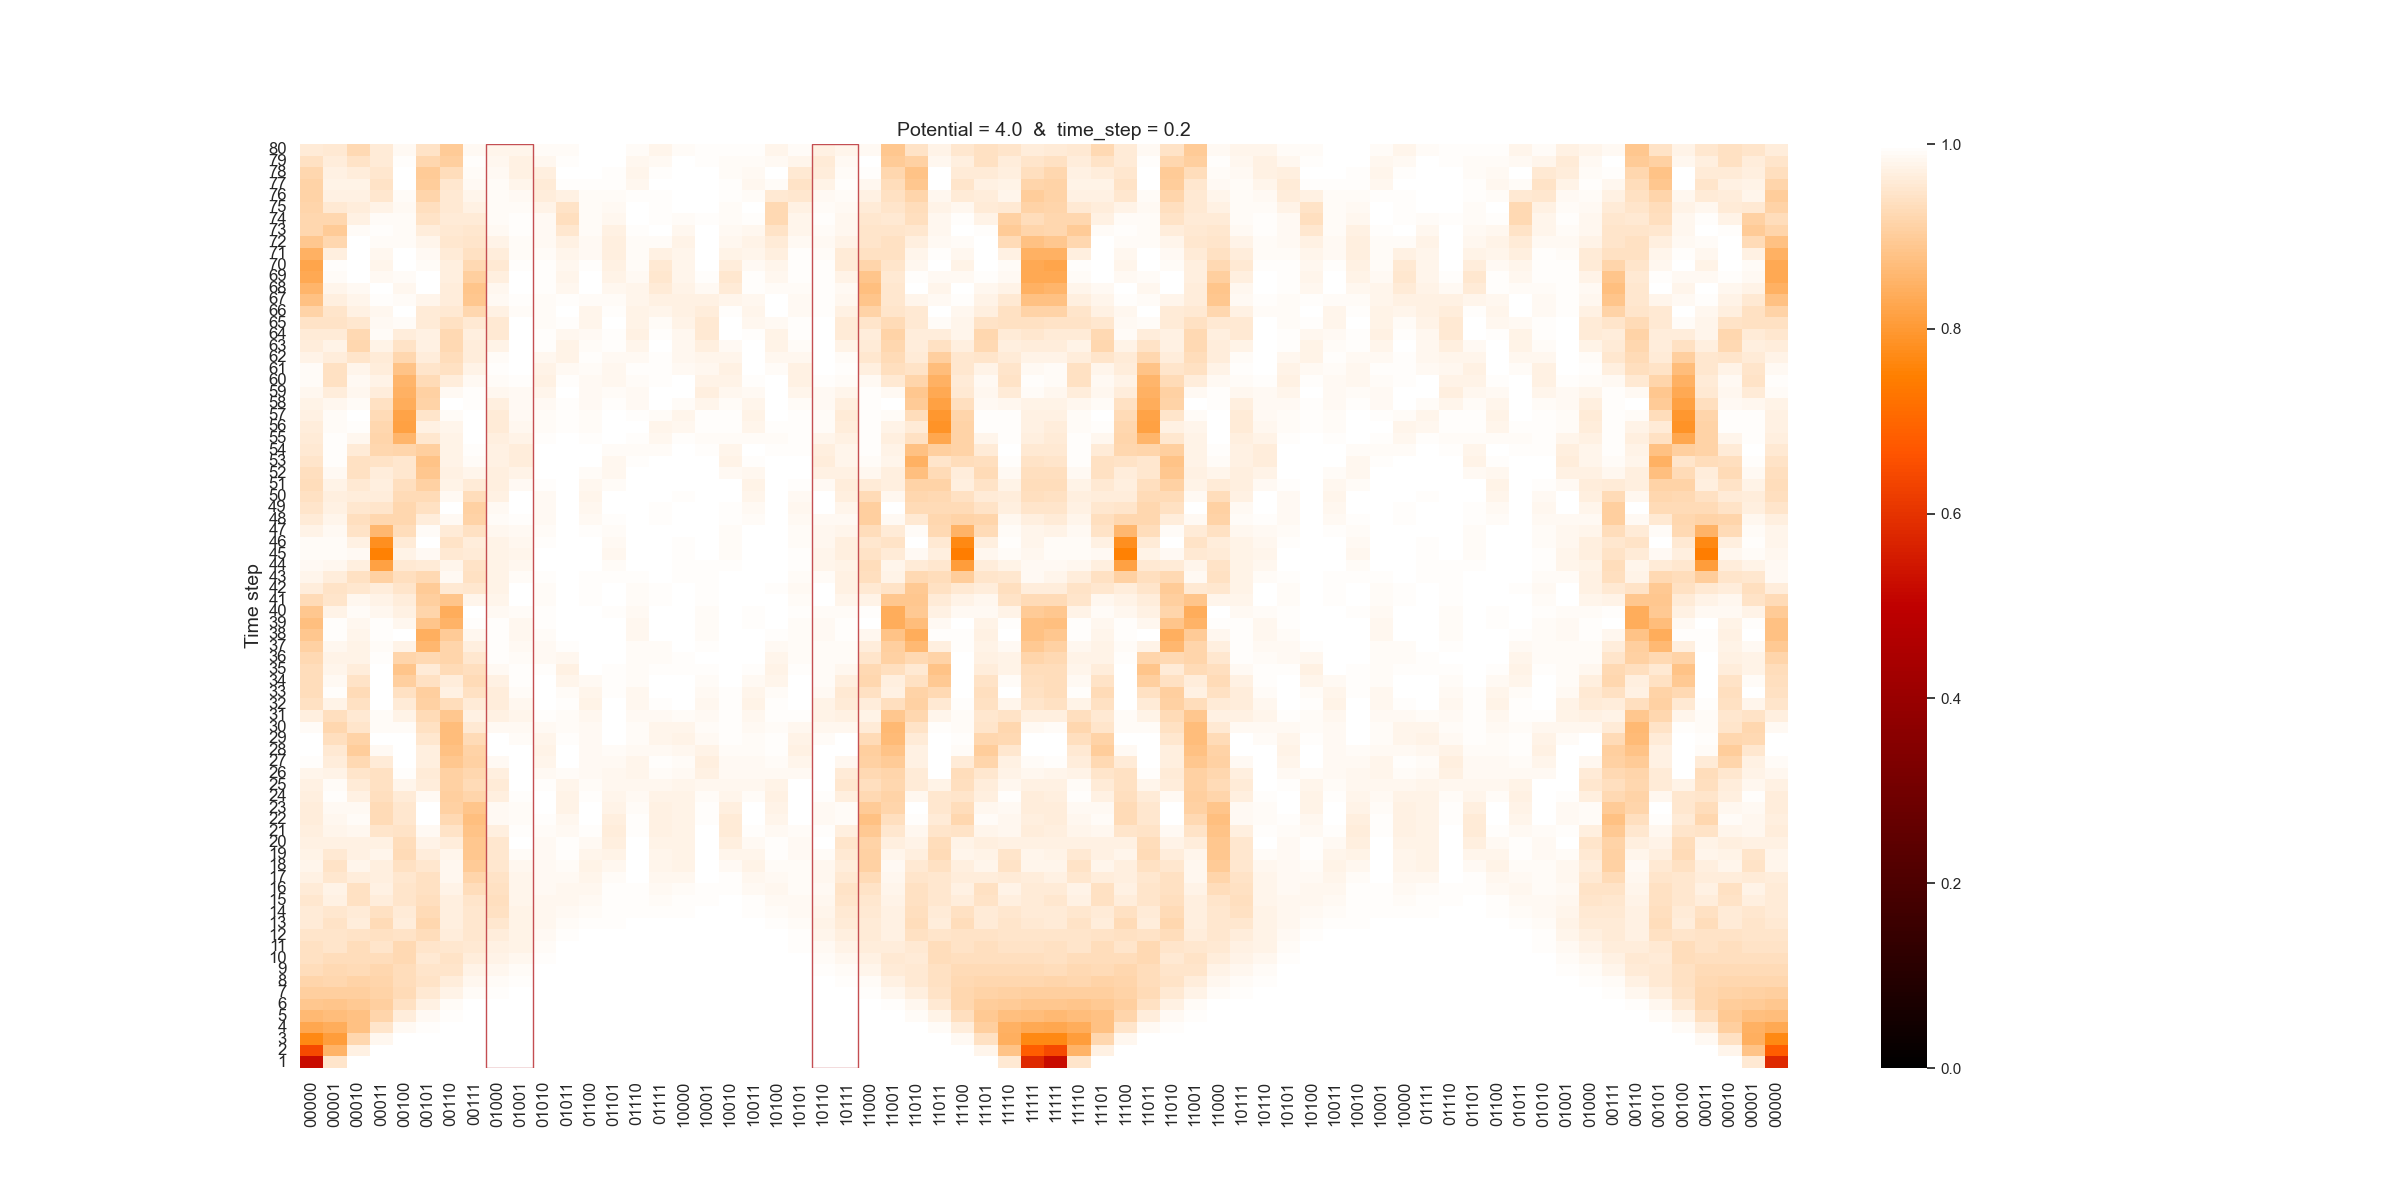
\includegraphics[width=0.95\textwidth]{media/sym_8_v_4.0.png}
    \caption{
        The symmetric potential. }
    \label{fig:quantum_tunneling_simulation}
\end{figure}

\begin{figure}
    \centering
    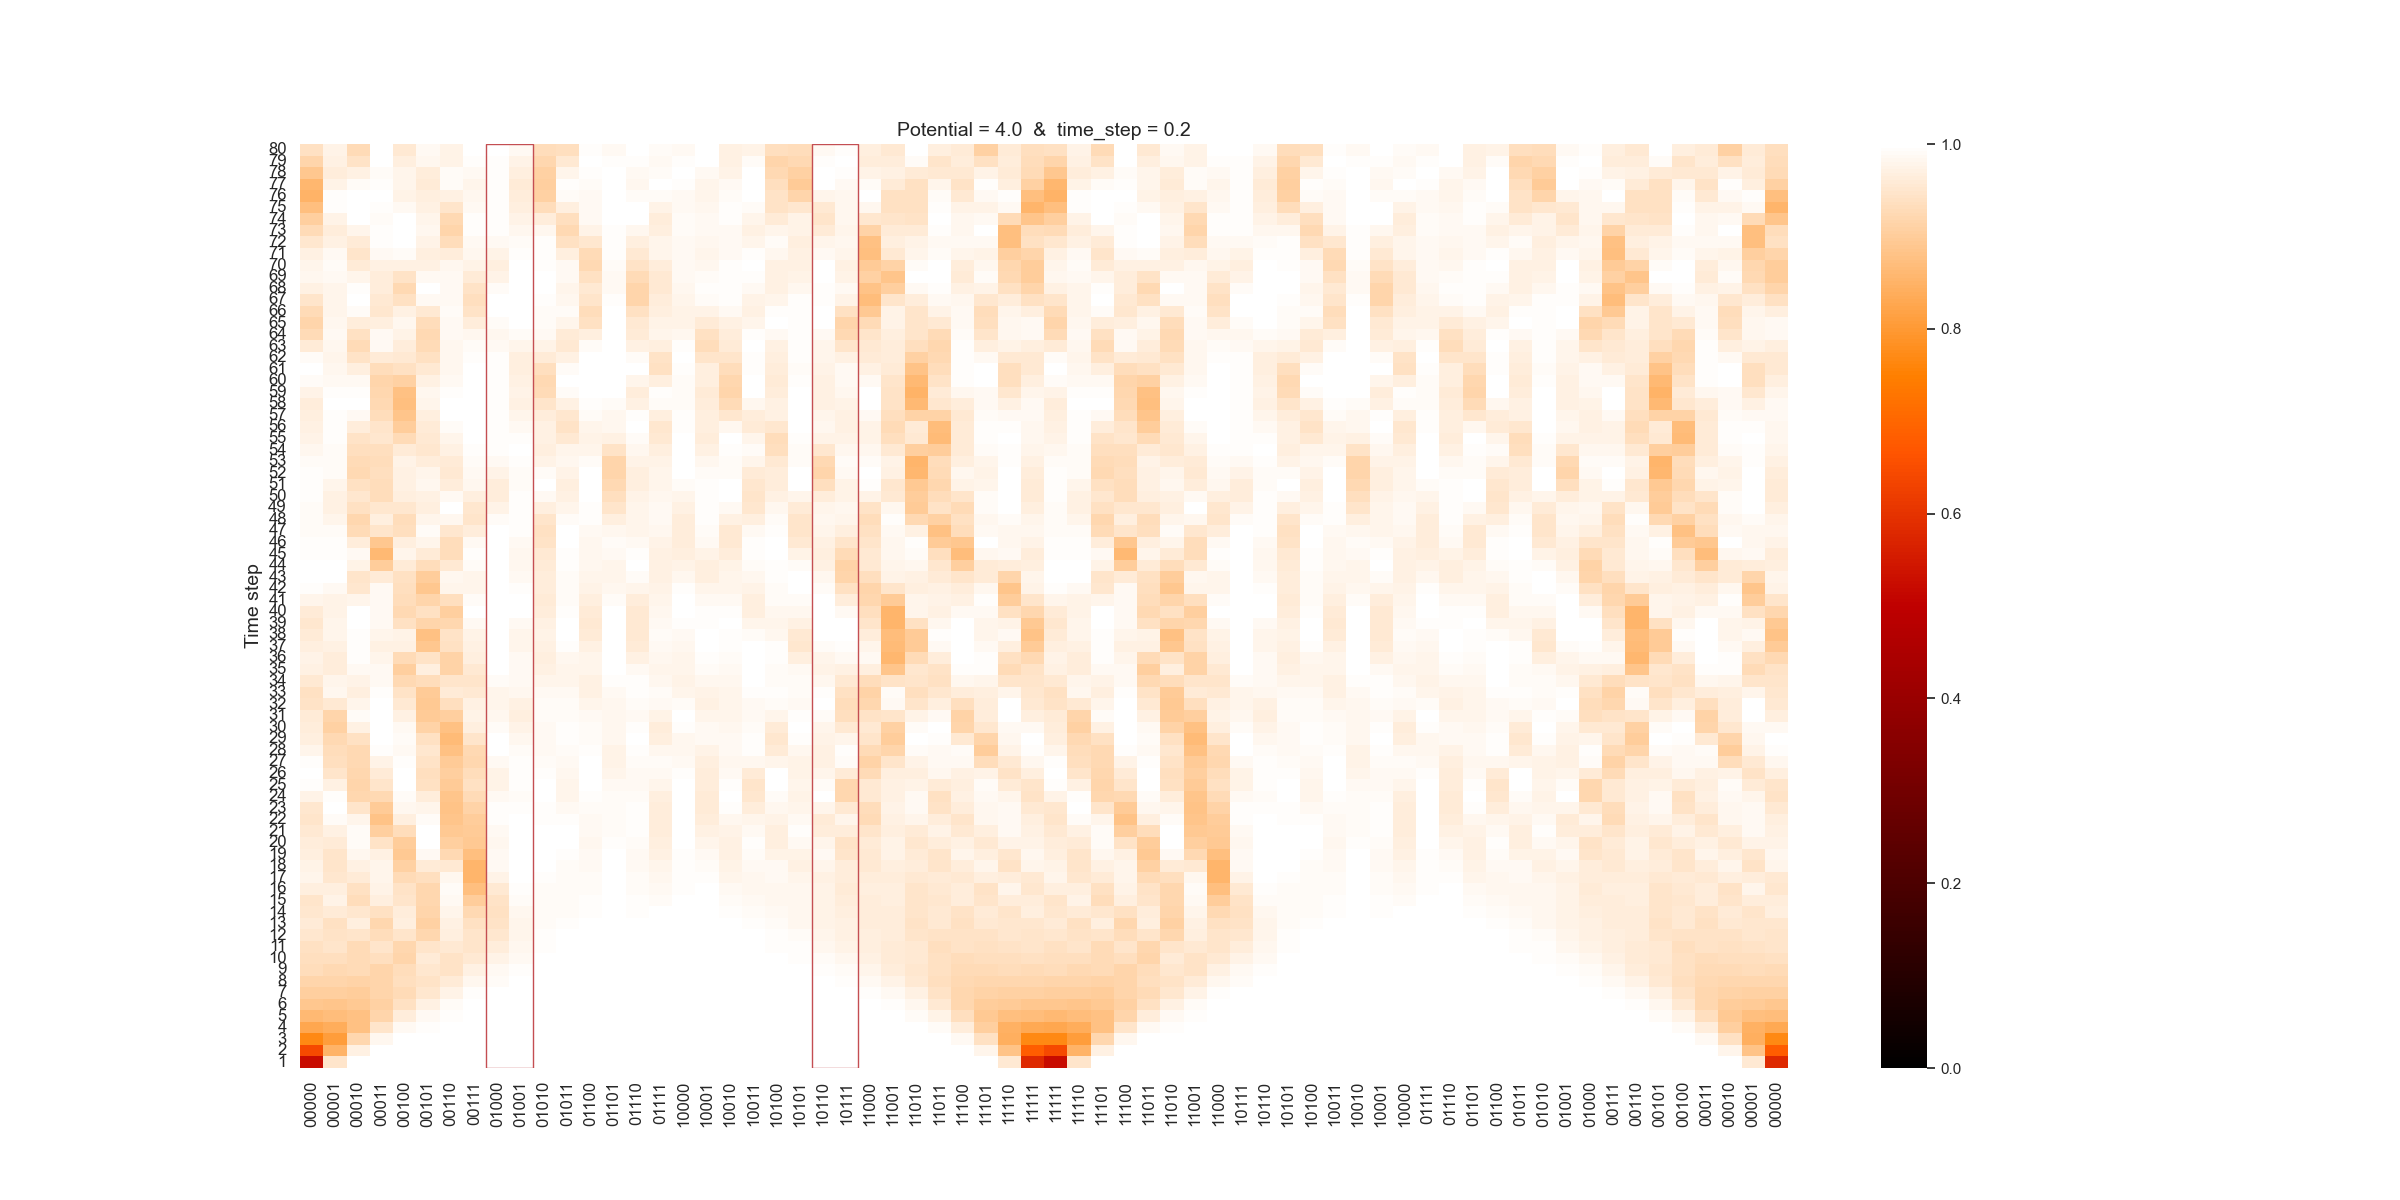
\includegraphics[width=0.95\textwidth]{media/asym_8_v_4.0.png}
    \caption{
        The reduced the right potential as $1/4$ times of the left potential.}
    \label{fig:quantum_tunneling_simulation2}
\end{figure}

\subsection{Slite experiment}
Using a tunneling circuit and 
the time dependent Hamiltonian, the Slit experiment 
could be simulated with  quantum computer where the time $t$ 
indicate the position $x$, the axis where particle is moving.
\subsection{}

\chapter{Adiabatic process on gate model}

Adiabatic computation


In practical implementation, adiabatic model of quantum computation
has many advantages in scale, speed and formulation of problem to run on the system.
On the gate model, we consider many approximation formula and representation of the evolution operator. 
The reason was that we cannot know exactly what form of the time-evolution operator form corresponding to the given hamiltonian matrix;hermite. 
However, in adiabatic computation, the unitary transformation is a \textbf{job of nature}. 
Only things we have to consider are how to apply the Hamiltonian to the given qubit system and 
accelerating convergence speed enough to use in calculation.
This computation model has very huge benefit in binary optimization problem than the gate model computation.

In this chapter, we are going to simulate adiabatic
process on gate model computer and compare the result obtained
from a commercial adiabatic process machine.

\section{Formulation for Adiabatic computing}

Adiabatic theorem states that if the system hamiltonian is varying slowly, 
the final state of the system is remained in eigenstate of finial hamiltonian 
which is corresponding eigenstate of the initial hamiltonian eigenstate.

The term slowly is very important, it depends on the initial and final hamiltonian of the system. 
If the evolution time is $T$, and the eigenvalues of initial and final hamiltonian are $E_i$
and, $E_f$, the evolution time must satisfy next,

\begin{equation}
    \frac{2 \pi}{|E_f - E_i| << T}
\end{equation}

That is to solve the system with adiabatic method, we have to manipulate the time, $T$.
It is called by \textit{adiabatic configuration}. 
The configuration depends on the initial and final system, 
so the determination requires some physical intuition by the researcher.

\begin{equation}
    \mathcal{H}_{adia} (f(s), T) = T(1- f(s)) \mathcal{H}_{initial} + f(s) \mathcal{H}_{solve}
\end{equation}

Our major concern is a ground state of $\mathcal{H}_{solve}$.
We can expect the system to be a ground state through adiabatic process,
if the initial system state was a ground state of $\mathcal{H}_{inital}$.
That is, with adiabatic process, we can obtain the target system ground state 
using well-known system.
The requirement is an appropriate Hamiltonian, $\mathcal{H}_{initial}$.
It must have well-known ground state and 
their implementation should practically be efficient.
Common Hamiltonian is a $\mathcal{H}_{inital} = - \sum_{i} \sigma_{X, i}$.
Its ground state is a $|+\rangle^{\otimes n}$.

\begin{center}
    \begin{quantikz}
        \lstick{$| 0_{0} \rangle$} &\gate{H}& \rstick{$| + \rangle$}  \\
        \lstick{$| 0_{1} \rangle$} &\gate{H}& \rstick{$| + \rangle$} \\
        \wave&& \\
        \lstick{$| 0_{n} \rangle$} &\gate{H}& \rstick{$| + \rangle$}
    \end{quantikz} = $|+\rangle^{\otimes n}$
\end{center}

The common annealing solutions, such as D-Wave and QuEra, also apply the adiabatic theorem to their initialization process and Hamiltonian form. 
Quantum annealing is fundamentally based on the phenomenon of quantum fluctuation; 
however, the starting and final stages, as well as the evolving process, follow the adiabatic theorem. 
That is why they offer some annealing time and initial state parameters to the user API. 
Some problems require much more time to achieve the appropriate adiabatic process

\section{Naive Implementation}

The previous simulations were time-independent
Hamiltonian systems, but adiabatic process is 
using a time-dependent Hamiltonian.
The commutation problem still arises in here.
If the $H(t_1)$ and $H(t_2)$ are not commuting, 
then we cannot apply the usual exponential formula.

Still, product formula work well except the additional error 
term was added to the system.

We can approximate this process with generating step Hamiltonians as 

\begin{equation}
    H_qc(t) = \left( 1- \frac{t}{T}\right) \mu H_i + \left( \frac{t}{T}\right) H_{solve}
\end{equation}

where, $\mu$ is a wieght coefficient of initial state.

%\begin{algorithm}
%    \caption{Adiabatic Process Approximation}\label{alg:naive_adiabatic}
%    \begin{algorithmic}
%    \Require $H_i, \mu, H_f$ \Comment{Initial Hamiltonian}
%    \Ensure $y = x^n$
%    \State $y \gets 1$
%    \State $X \gets x$
%    \State $N \gets n$
%    \While{$i < step$}
%    \If{$N$ is even}
%        \State $X \gets X \times X$
%        \State $N \gets \frac{N}{2}$  \Comment{This is a comment}
%    \ElsIf{$N$ is odd}
%        \State $y \gets y \times X$
%        \State $N \gets N - 1$
%    \EndIf
%    \EndWhile
%    \end{algorithmic}
%    \end{algorithm}

\begin{lstlisting}
    [Adiabatic Processs Approximation]

    H_i <- initial hamiltonian
    mu <- weight of the H_i
    H_f <- problem hamiltonian
    --------------------------------------------------
    func_evolve(t, H, tn): 
        Applying time evolution operator on state
            evolution time: t, 
            hamiltonian: H 
            trroter decompose level: tn.
    
    func_Hqc(s, t, mu): (1-s/t) mu * H_i + (s/t) H_f
        Return instaneous hamiltonian of the given time step: s.
        --------------------------------------------------
    [Defined Adabatic schedule parameters]
    
    T <-  # total evolution time
    steps <-  # time difference step number
    dt <- T/steps
    
    trotter_num <- # trotter decompose level
    
    [Prepare the circuit]
    
    initiate the system with Hadamard basis |+>
    
    while i < step
        t = dt*i
        H_t = func_Hqc(t, T, mu)
        ----------------
        func_evolve(dt, H_t, trotter_num)
    
    Sampling, Measure Expectation Value ... et cetra
\end{lstlisting}


\begin{example}[Problem Modeling]
    In this example, we refer a simple NP-hard problem.
    It is finding a source distribution producing flat radiation.
    
    \begin{center}
        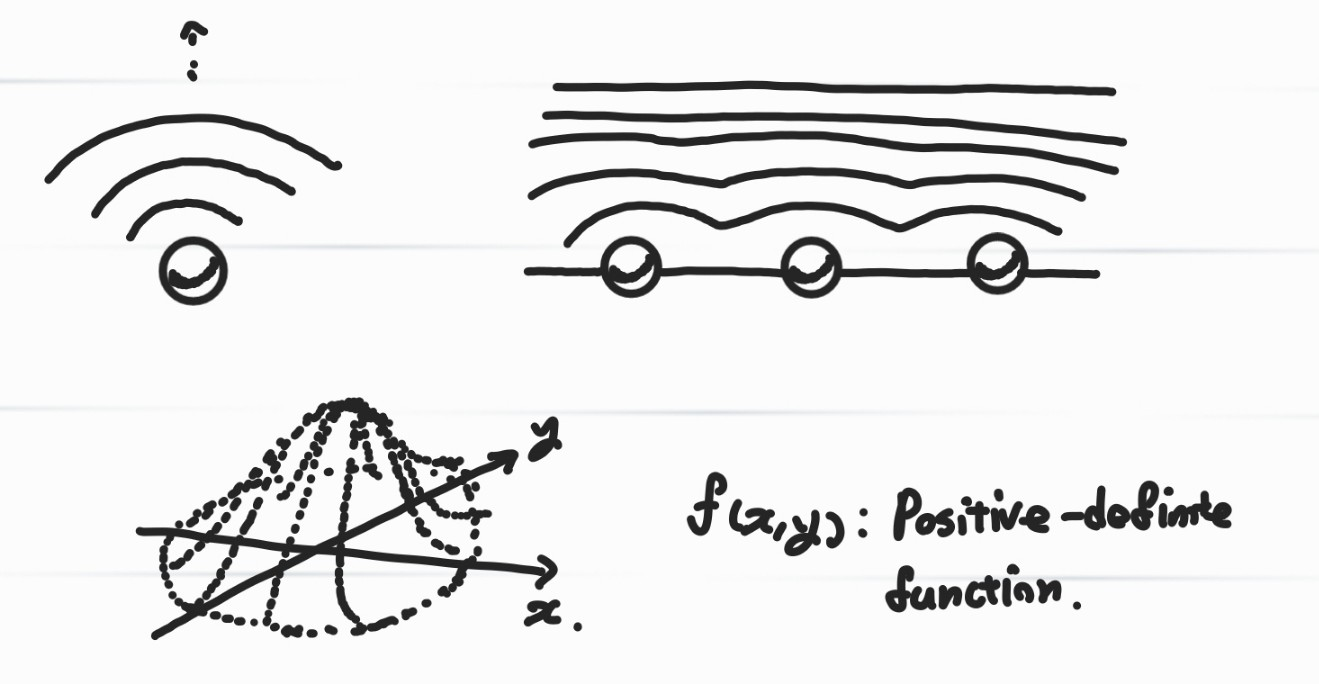
\includegraphics[width=0.8\textwidth]{media/source_distribution.jpg}
        \captionof{figure}{Source optimization problem.}
    \end{center}
    % Matrix -imshow, 
    %

    \begin{itemize}
        \item Radiation on the given surface = $\mathbf{r}$
        \item Propagation matrix = $K$
        \item Source distribution: $\mathbf{x}$, binary vector
    \end{itemize}
    
    \begin{equation*}
        K\mathbf{x} = \mathbf{r}
    \end{equation*}
    
    We want to obtain a flat radiation to some area far from the source plane, so let us apply difference matrix to both term. 
    If flatness is achieved, then the right term would be zero.

    The radiation function is $f(x) = (1+ x^2)^{-1}$
    This problem could be converted to a quadratic optimization problem by next equation.
    \begin{equation}
        \min \mathbf{x}^T A \mathbf{x}
    \end{equation}
    where, $A = Q^TQ, Q = D K$.
    The optimal solution is 
    \begin{equation*}
        \mathbf{x}_{opt} = \begin{bmatrix}
            1& 1& 0 & 1 & 0 & 1& 1&
        \end{bmatrix}
    \end{equation*}
    Since, $A$ is Hermit matrix so that we can interpret it as givein Hamiltonian.
\end{example}

You can refer a Pennylane and D-Wave implementation code of the result written by the author\cite{Kim_adiabatic_implementation}.

\subsection{Example QUBO}

Quadratic unconstrained binary optimization problem.
It is widely tried in adiabatic computation and 
in gate-model computation VQE(Variational Quantum Eigensolver) method is 
dominant however, in this chapter we will solve the 
QUBO problem on gate model computer mimicing the adiabatic process.




\begin{equation}
    D K \mathbf{x} = D \mathbf{r} = 0
\end{equation}





\subsection{Ising model}

\section{Pennylane implmentation}

\subsection{Graph partitioning problem}




\chapter{Imaginary Time evolution}


\section{Imaginary time}

Imaginary time evolution is frequently used in 
quantum system simulation especially, in statistical 
physics. 
In the statistical mechanics it is called by 
\textit{Diffusion Montecarlo method}. 
The reason is that from the Schr$\ddot{\mbox{o}}$dinger equation,
we can directly obtain a progress to reach the ground state of the system.
From the time-independent Schr$\ddot{\mbox{o}}$dinger equation, 

\begin{equation}
    i \hbar \frac{\partial}{\partial}| \psi \rangle = H |\psi \rangle
\end{equation}

takes $\tau = i t$  then, $df/d\tau = (dt/d\tau) df/dt = i df/dt$, thus,

\begin{align}
    \frac{\partial}{\partial \tau} | \psi \rangle = H | \psi \rangle \label{eq:imginary_sch_eq}\\
    | \psi(\tau) \rangle = e^{- \tau H} | \psi(0) \rangle
\end{align}

From the Eq (\ref{eq:imginary_sch_eq}), we get a general solution,

\begin{equation}
    |\Psi \rangle = \sum_{i} c_i(0) e^{- E_i \tau} | \psi_i \rangle
\end{equation}

The terms are decaying and does not oscillate. Therefore, with sufficient long time, $\tau$, 
we get 

\begin{equation}
    |\Psi(\tau) \approx_{\tau \rightarrow \infty} c_g(0) e^{- E_g \tau} | \psi_g \rangle
\end{equation}

However, the imaginary time evolution cannot be directly 
implemented in common gate model computer. 
Since, it is a non-unitary transformation, $\exp(-H \tau)^\dagger = \exp(-H \tau)$, Hermit. 
Therefore, the implementation of ITE is also a challenge in the quantum computation.
There are several ways, one is approximate the non-unitary gate with unitary gate.
It is a common method by VQE, we can approximate unitary process to reach the same result 
of the imaginary time steps. 
The other methods are a block-encoding, embeding the non-unitary gate into unitary gate, or
using a measurement based approach. 
The method we used in the implementation was non-unitary Trotter circuit suggested by Leadbeater et al\cite{leadbeater_non-unitary_2023}.
Once we get a proper ITE routine, then the quantum computer could find a ground state from 
the \textit{given} states.

\section{Non-unitary on unitary}

There are many method to obtain non-unitary
operation on unitary system.
\subsection{Embeding in unitary}

Even the whole gate was unitary,
their sub-block matrix could be non-unitary.
Using an ancilla register, we can obtain a
non-unitary operation on the main register.

Especially, the measurement based 
operation suggested by 
is based on Trotterization.


\subsection{VQE approximation}

\section{Spectrum Search}
\chapter{Variational method}

It is considered practically useful method in
NISQ era\footnote{Noisy intermediate scale quantum era}.


Review \cite{cerezo_variational_2021}.
\section{Introduction}

\subsection{Variatiaonal Principle}

\subsection{Circuit as ansatz}

The term \textit{ansatz} means an assumption 
in mathematics or physics to solve the given problem.
In the physics, it is commonly refer a model representing 
or containing the solution of the problem.
The statement of \textit{Is the ansatz proper to solve the problem?}
refers the whether is it possible that "The solution could be represented with the model"
or, in optimization problem, "The ansatz achive the desire solution".

Using a paramerized circuit, we can treat the quantum circuit 
as a neural network in machine leanring. 
However, if the result is not bounded, 
the optimization is meaningless for any kinds purpose.
That is why we need a \textit{Variational principle}.
Since, quantum circuit is a kind of quantum system and their
ground state and energy is limited in finite value.
Same statement holds for parameterized circuit, there always 
exists a ground state energy\footnote{Not a state. There could be degenerated states.}.

Whatever energy we measure from quantum circuit, it is always higher or equal with the ground state.

\begin{equation*}
    E_{ground} \leq \langle \psi | H | \psi \rangle
\end{equation*}


We can optimize the circuit without any worry about their convergence.


\begin{principle}
    \textbf{Variational Principle}

    \begin{equation}
        E_{g} \leq \langle \psi | H | \psi \rangle \leq E_{\mbox{max}}
    \end{equation}
\end{principle}

\subsection{Universality of Circuit}

One of the strong background of the neural network model is 
\textit{Universal Approximation Theorem}. 

How about quantum circuit? Do we have any those type of theorem?
The answer is yes!. Quantum circuit is also a universal approximator.
In addition, it is more powerful. Even with a single qubit we can achieve the property\cite{PhysRevA.104.012405-Universal-approxi}.

\section{}

\section{Ansatzs}

\subsection{Hardware Efficient}

\subsection{Evolution Based}


\section{Application}

\subsection{QUBO}

\subsection{Evolution}

\subsubsection{Real time}

\subsubsection{Imaginary time}

\section{Implementation}

\subsection{Pennylane}

\subsection{Qiskit}

\bibliographystyle{unsrt}
\bibliography{vqe}


\chapter{Material Simulation}


\section{Hardness of the simulation}

Degree of freedom is high enough
\chapter{Tunneling Phenomenon}

Quantum tunneling is one of non-classical phenomenon in real-world with entanglement and wave-particle duality.
Suppose that the free particle of $m, p$ mass and momentum pass through a potential varrier, $V$ in 1-dimension.

\section{Introduction to tunneling}

\begin{figure}
    \caption{}
    \label{fig:tunneling}
\end{figure}

The solution of the Schr$\ddot{\mbox{o}}$dinger  equation yields,

\begin{eqnarray}
    \psi(x) = A \exp(\pm ikx)
\end{eqnarray}


The tunneling effect arises in the situation when $E <V$. 
In classically, at the $b<x$, the existence possibility of the particle is zero.
However, it is not in quantum mechanics


\subsection{alpha-decay}
The tunneling effect successfully explained the \textit{alpha}-decay phenonmenon by George Gamow, and Condon and Gurney, indepedently.
In the Columb potential of the nuclear, 
the alpha particle cannot obtain the enough energy 
to escape the nuclear binding force.
However, in many experiment and observation alpha particle emission was occured

\section{Tunneling time problem}

\begin{definition}{\textbf{Tunneling time problem}}

    How many time does it take to pass through the potential region, when the tunneling effect is occurred?
\end{definition}

This simple question has not been solved yet.

\section{Criticisims on tunneling time}

The major problem is that there does not exist about some common definition of \textit{time} in quantum mechanics.
Time is just a parameter in quantum mechanics, meanwhile, in general relativity, spacetime dynamically interacts with matters.  

Imaginary time evolution problem: Imaginary number has no proper order by the definition. 
How can we define proper flow direction of time in imaginary numbers?

There are some definitions of tunneling time.
The concepts have their own criticisims about how they well explain the tunneling time problem, 
however, they are practically used in required field, such electrodynamics.

\begin{enumerate}
    \item Dwell-time
    \item Wignet-time
    \item Larmor-time
\end{enumerate}

A proper time observable, $T_c$, should satisfy the following properteis:

\begin{enumerate}
    \item On average $T_c$ should estimate te elaspsed time $\tau$.
    \item The variance in a measurement of $T_c$ should be independent of the elapsed time $\tau$.
\end{enumerate}

\subsection{Classical approach}

In the classsic scale, the potential is simply a hill. 

\subsection{Measurement- Experimental}

\subsubsection{Larmor Precession}

The spin is rotated in the uniform magentic field, $B_0 \hat{z}$ with constant frequency $\omega$. 
Such phenomenon is called \textit{Larmor precession} and the frequency is called \textit{Larmor frequency}.
If the particle is 

\subsection{Hartman effect and Superluminal velocity}

Hartman effect


\section{Simulation and Measurement on Quantum circuit}

Consider Larmor precession implementation on quantum circuit. 
The spatial propagation of 1 dimension is well established at section \ref{sec:1dim_particle}.
If we want to implement Larmor precession, 
we can add an additional qubit to act as a spin of the free particle,
and modifying the Hamiltonian adding spiner term. 
Does it really a good simulation? Why we do a calculation and simulate the phenomenon on circuit?
We want to obtain a complex system behavior through the simulation, 
however, designing an affecting circuit to such qubit by time-evolution effect 
is itself a problem we want to solve. 
In experiment, it could be a good clock system for the tunneling phenomenon.
Meanwhile, in simulation, we cannot get a meaningful information from the model.

In addition, it is just a extracting time\footnote[4]{Maybe events} information from the system register.
Why it must be Larmor time depending on only a specific potential; magenetic potential.
Tunneling is an universal phenonmenon that does not depends on the types of potential.
A good clock simulator must act on the general situation whatever potnetial type it is.

\subsection{Page Wootter Mechanics}

The previous definitions of clock and time of tunnleing effect were based on the wave function, 
probability current and their change by the time.

We are focusing on the situation of \textbf{the event occurred} stuation.
The particle occurrence proability of the given space is closely related with the event occurrence.
However, there is a gap between the stuations. 
Unfortunately, in the common Schr$\ddot{\mbox{o}}$dinger  equation cannot handle the case of our attention.
It is because the Schr$\ddot{\mbox{o}}$dinger  equation didn't consider the relativity, so that the time is \textit{not an observable quantity}.
The dynamical interaction of space time with matter is described by general relativity.
Related with gravity and quantum system. 

However, Dirac/canonical quatization of gravity yields \textit{Frozen Formalism}\footnote{It was impeorted from , Smith, Aleander, "The Page-Wootters formalism: Where are we now?", 10.48660/22010079}. 
General realtivity can be represented with Hamiltonian form as Eq (\ref{eq:ge_hamiltonian}).

\begin{align}
    H_{GR}[\gamma , P] = 16 \pi G  G_{abcd}[\gamma] P^{ab} P^{cd} + V{\gamma} + \sqrt{\gamma} \rho =0 \label{eq:ge_hamiltonian}\\
    H_{GR} | \Psi \rangle = 0\\
    i \frac{d}{d t} | \Psi \rangle = H_{GR} | \Psi \rangle = 0
\end{align}

What does the above equation means? The state vector $| \Psi \rangle$ is frozen which means there is no evolution.
This is gravitation quantization problem related to the problem of time.

However, recently, there is a re-splotlighted perspective of quantum time in the field which has been known as 
\textit{Page-Wootter formalizm}. In 1983, Page and Wootters presented extended version of the equation\cite{PhysRevD.27.2885}. 
This is called PaW mechanics.
PaW mechanics treat the time as a quantum degree of freedom in specific Hilbert space, and 
in the viewpoint, time flow is occurred from the entanglement between such space and the remained physical system.
There were some critisim about the formalization of PaW mechanics;proper propagator, ... .
Giovannetti technically reformalize the PaW structure and showed PaW mechanics can be extended 
to give the time-independent Schr$\ddot{\mbox{o}}$dinger  equation\cite{PhysRevD.92.045033}.


\subsubsection{Evolution as a basis change}

The evolution is an unitary transformation, and 
every unitary transformation is a kind of basis transformation.
Even the overall state is frozen by the time. 
The basis change does not affect the static state,
however, locally there could be a dynamics.

\subsubsection{Structure of PaW mechancis}

The system, $\mathfrak{H}$ is consist of Hilbert space of the ordinary system, $\mathcal{H}_s$ and ancillary Hilbert space, 
$\mathcal{H}_T$, of clock or time.

\begin{eqnarray}
    \mathfrak{H} = \mathcal{H}_T \otimes \mathcal{H}_S
\end{eqnarray}

\begin{eqnarray}
    \hat{\mathbb{J}}  = \hbar \hat{\Omega} \otimes \mathbf{1}_S + \mathbf{1}_T \otimes \hat{H}_S \\
    |\Psi \rangle \rangle = \int dt | t \rangle_T \otimes | \psi(t) \rangle_S \\
    \hat{\mathbb{J}} | \Psi \rangle\rangle = 0 
\end{eqnarray}

From unitary time evolution operator on the system, $\hat{U}_S(t)$ we can construct a proper evolution of the system.

\begin{eqnarray}
    \mathbb{U} &=& \int dt | t \rangle_T \langle| \otimes \hat{U}_S(t) \\
    &=& \hat{U}(\hat{T}) = \exp(- i \hat{T} \otimes \hat{H}_s /\hbar) 
\end{eqnarray}


The main benefit of the PaW mechanics is that the time is an observable quantity in the mechanics and 
we can obtain a basyian probability on time-dimension about the occurred event following Boron's rule.

\begin{equation}
    P(A |B) = \frac{\mbox{tr}(P_A P_B \rho P_B) }{\mbox{tr}(P_B \rho P_B)}
\end{equation}

In the approach, the author treating the quantum tunneling time on the analysis of \textit{arrival time}.

The goodness of the PaW mechanism is that it can be directly implemented on quantum circuit by ancilla qubit registers.
The pure state is well-suited with qubit network and 


%===================================
\newpage
\part{Further Topics}
\section{Simulation Techniques}

\subsection{VQE evolution}
VQE is an abbrevation of Variational Quantum Eigensolver.

In qiskit, they offer two type of evolution modules. 
One is a Product formula based implementation we already described in the previous contents.
The other is a VQE based module that is called Variational quantum time evolution.

The theorem is based on the paper written by Yuan et al\cite{yuan_theory_2019}, 

\subsection{Linearization}

\subsection{Quantum Walks}

\subsection{Qubitaization}

\subsection{Fractional Query}

\subsection{Taylorization}
%======================================================================================================================================
\newpage
\bibliographystyle{unsrt}
\bibliography{references.bib}

%======================================================================================================================================
\newpage
\part{Appendix}
\appendix

\chapter{Hermit and Unitary matrix}
\label{appendix_chap:hermit_uni}
\section{Unitary matrix}

Let's think about there is a change, whatever it is, in the system.
The $| \psi \rangle$ represent all the information of the system, so that it will be changed to $| \psi' \rangle$. 

Any modification in the vector space can be represented with an \textit{operator}, $\hat{U}$.

\begin{equation}
    |\psi' \rangle = \hat{U} | \psi \rangle
\end{equation}

Now, the modified state function also satisfies normalization, such as $\langle \psi' | \psi \rangle = \langle \psi | \psi \rangle$.

\begin{eqnarray*}
    \langle \psi' | \psi \rangle = \langle \hat{U} \psi | |\hat{U} \psi \rangle \\ 
    \langle \hat{U} \psi | |\hat{U} \psi \rangle = \langle  \psi| \hat{U}^{\dagger}|\hat{U} \psi \rangle\\
    \langle \psi| \hat{U}^{\dagger}|\hat{U} \psi \rangle = \langle \psi| \hat{U}^{\dagger}\hat{U}| \psi \rangle
\end{eqnarray*}

we get,

\begin{equation}
    \label{eq:unitary}
    \hat{U}^\dagger \hat{U} = \hat{I}
\end{equation}

where, $\hat{I}$ is an identity operator. 

That means that any state change event in the quantum system must be a unitary operator in vector space, in isolated system.
With well defined basis, we can formulate the operator as matrix, 

\begin{eqnarray*}
    {|\Psi \rangle} &= {\sum c_i |\psi_i \rangle} \\
    {[\hat{U}]}_{\psi_i} &= \sum (\langle \psi_j | \hat{U} |\psi_i \rangle) |\psi_i \rangle \langle \psi_j|
\end{eqnarray*}

It is little bit weired that the function operation as a matrix, however, we are treating basis function that generating all functions.
About the those set of functions we can find well-ordered basis, of course it does not have to be finite.
Even in the infinite dimensional vector space, we can find a subspace consist of discreted index basis.
Think about the Fourier series of the $L$ periodic function. 
The basis functions are $\cos(\lambda_n x), n \in \mathbb{Z}_+ $.

That is why the unitary matrix is essential topic in quantum computation and simulation.

\subsection{Properties of unitary matrix}

\begin{itemize}
    \item It preserves the inner product of two vector, $\mathbf{x,y}, \langle \mathbf{x |y }\rangle = \langle U \mathbf{x}| U \mathbf{y}\rangle$
    \item It is a normal operator: $A A^\dagger = A^\dagger A$.
    \item $U^\dagger = U^{-1}$
    \item There exists a Hermit matrix $H$ such that $U = \exp(i H)$.
    \item Eigenvalues are \textit{unimodular} which is their norms are 1. Therefore, $|\det(U)| =1$.
\end{itemize}

In quantum systems symulation, 
finding a proper unitary operation on system is a significant work.
In sometime, we only focus on the result of the operation, in that case 
we can find some equivalence unitary operators with less implmentation cost.

In the property of the unitary matrix, there is $U = \exp(i H)$. 
It is a very familiar term in quantum mechanics; time-evolution operator. 
In finite dimension, the Hamiltonian, $H$, is represented by \textit{Hermit} matrix.

\section{Hermit matrix}

Suppose the Hamiltonian of the system is given as $H$. The Schr$\ddot{\mbox{o}}$dinger  equation yields next.

\begin{equation}
    i \hbar \frac{d}{d t} | \psi \rangle = H | \psi \rangle
\end{equation}

Hamiltonian is a kind of operator of measurement for energy of the system. 
It means that the eigenvalues of matrix are energy of the eiegenstates.
Such that 

\begin{equation}
    \hat{H} | \psi \rangle = E | \psi \rangle
\end{equation}


\begin{eqnarray}
    \langle \psi | \hat{H} | \psi \rangle = \langle \psi | |\hat{H}\psi \rangle = \langle \hat{H} \psi | | \psi \rangle \\
    \langle \psi |\hat{H}^\dagger | \psi \rangle = E^{\*} \langle \psi | \psi \rangle = E \langle \psi | \psi \rangle \\
    \therefore E^{\ast} = E
\end{eqnarray}

$E^{\ast} = E, \forall E$, the only complex value satisfying this constraint is a real value.
It means that the all eigenvalues of the matrix are real value.
Such matrices are called self-adjoint matrix or \textit{Hermit matrix}.

The definition of self-adjoint matrix is 

\begin{equation}
    H^\dagger = H .
\end{equation}

It is equivalence to the all eigenvalues are real condition.

We refered a Hamiltonian as an example of measurement, 
however, any measurement quantity operators are represented with Hermit matrices.
We call them as \textit{observable}.

\subsection{Properties of Hermite matrix}

\begin{itemize}
    \item All eigenvalues are real value.
    \item It is a self-adjoint matrix.
    \item All eigenvector having different eigenvalues are orthogonal to each other.
    \item Normal matrix.
    \item Closed under addition.
    \item If the two Hermite matrices are commute each other, then their product is Hermite matrix.
\end{itemize}

\begin{theorem}{Spectrum Theorem of Hermit matrix}
    \label{theorem:hermit_spectrum}
\end{theorem}
\section{Additional properties}

\begin{theorem}{\textbf{Diagonalizability of Hermit matrix}}

    For a given $H$ matrix, there exists an unitary matrix, $U$ such that 
    \begin{equation*}
        H = U D U^\dagger
    \end{equation*}
    where, $D$ is a diagonal matrix.
\end{theorem}

There are some common misconcept of the diagonalizability of the Hermit matrix,
about the orthonormal basis of the Hermit matrix.
The questions are

\begin{itemize}
    \item Why do the orthonormal eigenvectors exist, since we cannot guarantee the singularity.
    \item How do we guarantee that the two eigenvectors sharing 
    same eigenvalues are orthogonal?".
\end{itemize}".

The two questions are related with a misconcept in linear algebra.
The diagonalizability is related with singularity, of course, 
but it is not equivalent. 
There are diagonalizable but singular matrices, considering a matrix of which an eigen value is 0.
\begin{equation*}
    \begin{bmatrix}
        0 & 0\\
        0 & 1
    \end{bmatrix}
\end{equation*}
In other word, physically, we can get a 0 energy state by modifying the potential of the system. 
Therefore, the first question is solved.
The second question is equivalent with the existence of the diagonal matrix
of Hermit matrix. Since, the unitary operator preserve the inner product, 
the existence of the diagonal matrix, standard basis, guarantees the orthonormal basis.
 

\begin{theorem}{\textbf{Eigenvector conservation}}

    For a given non-singular Hermit matrix, $H$, with eigen values and their corresponding eigen vectors, $(\lambda, \mathbf{v})$,
    \begin{equation*}
        H \cdot \mathbf{v} = \lambda \mathbf{v}
    \end{equation*}
    then, 
    \begin{equation*}
        e^{H} \mathbf{v} = e^{\lambda }\mathbf{v}
    \end{equation*}
\end{theorem}

\begin{proof}
    From the taylor representation of matrix exponential, 
    \begin{equation*}
        e^{A} = \sum_{n=0}^\infty \frac{A}{n!}
    \end{equation*}
    then, 
    \begin{align*}
        e^{H} \mathbf{v} &= \left[ I + H + \frac{1}{2!} H^2 + \dots + \frac{1}{k!}H^k + \dots \right] \mathbf{v}&\\
        &= \left[ I\mathbf{v} + H\mathbf{v} + \frac{1}{2!} H^2\mathbf{v} + \dots + \frac{1}{k!}H^k\mathbf{v} + \dots \right]& \\
        &= \left[ \mathbf{v} + \lambda\mathbf{v} + \frac{1}{2!} \lambda^2\mathbf{v} + \dots + \frac{1}{k!}\lambda^k\mathbf{v} + \dots \right]& \\
        &= \left[ 1 + \lambda+ \frac{1}{2!} \lambda^2+ \dots + \frac{1}{k!}\lambda^k + \dots \right] \mathbf{v}& \\
        &= e^{\lambda} \mathbf{v}&
    \end{align*}
\end{proof}

\begin{theorem}{\textbf{Unitary on exponential}}

    For given unitary matrix, $U$, 
    \begin{equation*}
        e^{U A U ^\dagger} = U e^A U^\dagger \text{.}
    \end{equation*}
\end{theorem}
\begin{proof}
    \begin{align*}
        e^{U A U^\dagger} 
        &=  I + U A U^\dagger + \frac{1}{2!} (U A U^\dagger)^2 + \dots + \frac{1}{k!}(U A U^\dagger)^k + \dots &\\
        &= U I U^\dagger + U A U^\dagger + \frac{1}{2!} (U A U^\dagger)^2 + \dots + \frac{1}{k!}(U A U^\dagger)^k + \dots& \\
        &= U (I + A + \frac{1}{2!}A^2 + \dots + \frac{1}{k!} A^k + \dots ) U^\dagger&\\
        &= U e^A U^\dagger
    \end{align*}
\end{proof}
\chapter{Notation in Quantum circuit}

\section{State}

Decimal Notation
Product Notation

\chapter{Fourier Trasnformation}

\section{DFT and FFT}

Practical implementation of the FFT algorithm is well described in 
\textit{GSL FFT Algorithm} \cite{brian_gough_2023_7898076}.

\section{QFT}

Quantum Fourier transformation is a Fourier transoformation 
defined on the finite group.

\begin{equation}
    \label{eq:qft_def}
    | \psi \rangle = \sum_{j=1}^n x_j | j \rangle \rightarrow_{QFT} \sum_{j=1}^n y_k | k \rangle
\end{equation}

where, $y_k = \frac{1}{\sqrt{N}} \sum_{j=0}^{N-1} x_j \exp\left( 2 \pi i j \frac{k}{N} \right)$

\begin{theorem}
    QFT is an unitary transformation.
\end{theorem}

\begin{proof}
Let, $\hat{T}$ be an QFT defined on Eq (\ref{eq:qft_def}),

\begin{equation}
    \hat{T}\left( \sum_{j=0}^{N-1} x_j | j \rangle \right) = \sum_{k=0}^{N-1} y_k | k \rangle
\end{equation}

\begin{align}
    = \sum_{k=0}^{N-1} \frac{1}{\sqrt{N}} \sum_{j=0}^{N-1} x_j \exp\left(2 \pi i j \frac{k}{N} \right) | k \rangle \\
    = \sum_{j=0}^{N-1} \frac{1}{\sqrt{N}} \sum_{k=0}^{N-1} \exp\left(2 \pi i j \frac{k}{N} \right) | k \rangle \langle j| x_j | j \rangle
\end{align}

thereby, we can formulate the operator, $\hat{T}$ as $|k\rangle, |j \rangle$ states.

\begin{equation}
    \hat{T} = \frac{1}{\sqrt{N}} \sum_{k=0}^{N-1} \exp\left(2 \pi i j \frac{k}{N} \right) | k \rangle \langle j|
\end{equation}


\begin{align}
    \hat{T} \hat{T}^\dagger  = \frac{1}{N} \sum \sum \exp\left(2 \pi i \frac{k}{N} (j - j') \right) |j' \rangle \langle j |\\
    = \sum_{j, j'} \left( \frac{1}{N} \sum_{k=0} \exp(2 \pi i \frac{k}{N} ( j- j') ) \right) |j' \rangle \langle j|\\
    = \sum_{j=0}^{N-1} | j \rangle \langle j' |  = \mathds{1}, \square \text{.}
\end{align}

\end{proof}

\section{QFT implementation on Circuit}

\chapter{Fast Pauli Element manipulation}
\label{appendix:FPPM}

Most of the Quantum processor using spin dynamics, so that the Pauli matrices and 
$n$-folded Pauli strings are major elements to analysis and to manipulation the system.
Common method to implement Pauli algebra is a matrix representation, for $l= 0, 1, 2, 3$.

\begin{equation*}
    \sigma_l \in \left\{ \begin{bmatrix} 1& 0 \\ 0 &1\end{bmatrix}, 
    \begin{bmatrix} 0& 1 \\ 1 &0\end{bmatrix},
    \begin{bmatrix} 0& -i \\ i &0\end{bmatrix},
    \begin{bmatrix} 1& 0 \\ 0 &-1\end{bmatrix} \right\}
\end{equation*}

Pauli elements of $n$ number of particle system are easily achieved by tensor product of the 
Pauli elements of single particle system. For $n$ number of $1/2$ spin particles, there are $4^n$ number of Pauli elements.

\begin{equation*}
    P^{(n)} = \otimes_{l=0}^{4^n} \sigma_{a_l}
\end{equation*}

where, $a_l = 0, 1, 2, 3$.
Since, tensor product is well established in matrix space as kronecker product,
we can manipulate and analysis the Pauli elements with matrix operations.
Mathematically, there is no huddle and any ambiguous to deal the elements in matrix form.
We can implement Pauli algebra in any number of particle system.

\begin{exercise}(Matrix representation of Pauli algebra)

    Show that the matrix representation of the above Pauli elements satisfy the next equations,
    For $i,j,k,l \in \{0, 1, 2, 3\}$,

    \begin{equation*}
        [\sigma_j, \sigma_k] = 2 i \epsilon_{jkl} \sigma_l
    \end{equation*}
    and
    \begin{equation*}
        \sigma_j \cdot \sigma_k = \delta_{jk} I + i  \epsilon_{jkl} \sigma_l
    \end{equation*}
\end{exercise}

\begin{exercise}(Orthonormality of $n$-fold Pauli elements)

    Using Hilbert Schmidt inner product and norm, show that the $n$-folded Pauli elements are form a complete basis of
    $M_{2^n}(\mathbb{C})$.
\end{exercise}

The problem arise in computational aspect. 
Matrix operation is proportional to the dimension of Hilbert space, however, the dimension grows exponentially, $O(2^n)$,
by the number of particle, $n$. When we want to calculate two Pauli elements we need $O(2^n)$ operations.
In addition, decomposing given Hamiltonian, constructing a Pauli element matrix are also growth exponentially.


\begin{align*}
    P_k = P_i P_j\\
    H = \sum_j \lambda_j P_j^{(n)} \\
    H \rightarrow_{decompose} \sum_j \lambda_j P_j^{(n)}\\
    H \leftarrow_{compose} \sum_j \lambda_j P_j^{(n)}
\end{align*}

\subsection*{Complexity of Matrix representation}

Assume that the multiplication and addition as same.

\begin{exercise}(Algebra complexity)

    For $n$-particle system, what is a time complexity to calculate $P_i P_j$ in matrix form?
\end{exercise}

In addition, if a Pauli element is given, can you directly determine what Pauli element in the Hilbert space?
Matrix elements gave you enough information to identify what element was it. 
However, It is hard to map the matrix to corresponding Pauli element.

\begin{exercise}(Decomposition)

    The standard process of Hamiltonian decomposition is using an inner product of Hamiltonian and Pauli elements,
    \begin{equation*}
        \lambda_j = \langle H | P_j^{(n)} \rangle_{HS} = \frac{1}{2^n} \tr(H^\dagger P_j^{(n)})
    \end{equation*}
    In $n$-particle system, what is a time complexity of single $\lambda_j = \langle H | P_j^{(n)} \rangle$ operation?
\end{exercise}

Let the answer of the above question as $f(n)$, then, since there are $4^n$ number of Pauli terms, 
the total complexity to decompose the Hamiltonian into Pauli terms becomes $O(f(n) 4^n)$.

\begin{exercise}(Composition)

    What is a time complexity to make a tensor product of two $n \times n$ and $m \times m$ dimension matrix?
    $n$ fold Pauli element is constructed by $n$ number of tensor product of $2 \times 2$ matrix.
    Calculate a time complexity to make a matrix form of single $n$-fold Pauli element by tensor product.
\end{exercise}

In the composition, we know the number of Pauli terms in the Hamiltonian.
Let the number as $k\in \{1, 4^n\}$. Then the total complexity is $O(k g(n))$. 
Therefore, the time complexity to make a matrix form of the given polynomial becomes at least $O(g(n))$, and 
maximally it becomes $O(4^n g(n))$. $g(n)$ would be an exponential value if you calculated well $g(n) \approx 8^n$. 

\section{Symplectic code representation}

Matrix representation is intuitive and easy to calculate, however, its computational complexity is poor.
In geometrical approach, researchers found that Pauli elements have a special property, \textit{symplectic}.
This interpretation gave us more convenience representation, \textit{symplectic representation}.

\begin{equation} 
    \label{eq:symplectic_pauli}
    P_j = (i)^f \hat{X}(a) \hat{Z}(b)
\end{equation}

Most of the quantum computing frameworks adopt symplectic code to manipulate the Pauli element efficiently.
There are requires mathematical backgrounds to understand the word symplectic and application in here
\footnote{Lie algebra, Clifford group and Differential geometry are required.}.
However, let us derive the result only with matrix and $\mathbb{Z}_2$ knowledges. 
If you are familiar with computational thinking, $\mathbb{Z}_2$ is just a classic bit manipulation.

$\sigma_0 = I, \sigma_1 = X, \sigma_2 = Y, \sigma_3 = Z$

\begin{example}(Symplectic representation in $n=1, 2$ Cases)

    $Y = -i XZ$
\end{example}
% Qskit, Pennylane, QuEra, PauliArray.




%-------------------
\subsection{Summary}

We can represent any Pauli elements

There are many references to deal the symplectic code, you can refer the code and documentations 
of quantum computing frameworks, such as Qiskit, Cirq, Pennylane, QuEra
%-------------------
\section{Acceleration of matrix conversion}

We solved the algebra complexity from exponential to linear degree. 
However, matrix conversion methods were not solved yet. 
Unfortunately, by the structure conversion between symplectic code and matrix 
could not be reduced to lower degree than exponential complexity.
Even though, we can reduce the complexity by reduce the base of the complexity, $O(k^n) \rightarrow O(l^n), l<k$.



The common decomposition is using Pauli terms, $H_i = P_{j(i)} = \Pi_{k} \sigma_l(k)^m$.
Since, Pauli terms form an orthonormal basis of the matrix space, 
the decomposition is well-defined on general $n$ qubit Hilbert space with 
Hilbert-Schmidt inner product.

\begin{equation}
    \lambda_i = \langle P_{j(i)} | H \rangle = \frac{1}{2^n} \tr(P_{j(i)} * H)
\end{equation}

The Pauli term representation is called \textit{Pauli-polynimial} of the given Hamiltonian $H$.
However, in large $n$, since the matrix dimension increases with exponential complexity,
the decomposition process requires huge computational resources 
in Hamiltonian analysis and Pauli-polynomial manipulation.

The time complexity of the matrix multiplication is $O(8^n)$, for $n$ qubit Hilbert space.
In addition, it is only about single Pauli term, so that the total coefficient cost is 
$O(32^n)$. It is because that we cannot know what terms are zero in the given 
Hamiltonian, and we have to test the all Pauli-terms.

Moreover, constructing the original Hamiltonian with matrix form
from the Pauli polynomial also arises in many situation.
Basic method is constructing each Pauli matrices with tensor products 
of 2-dim Pauli matrices, $\sigma_{i}, i \in \{0, 1, 2, 3\}$ 
and calculating a linear combination of them.
It is called \textit{term-by-term} method.
The complexity of term-by-term method rely on the complexity of 
single $n$-fold Pauli matrix term, $f(n)$,
and the number of non-zero terms in the polynomial, $k$.
Therefore, the complexity of the composition is $O(k(f(n) + 4^n))$.
There are $4^n$ number of Pauli terms, the worst case is $O(16^n + 4^n f(n))$.


\section{Decomposition}

\subsection{Tensorized method}


\subsection{Term-by-Term methods}

\section{Composition}
\subsection{PauliComposer}

\subsection{Inverse of the Tensorized method}

Since, the tensorized method is just a basis transformation, 
the inverse transformation is well defined, 
however, without the coefficient matrix of the Pauli-polynomial 
the inverse algorithm could not be used to construct the original 
Hamiltonian matrix. In the original paper by Hantzko et al \cite{hantzko_tensorized_2023},
they didn't find the way so that only mentioned about the decomposition method.

\begin{equation}
    \label{eq:restore}
    \begin{array}{ccc}
        c_0 &=& \frac{1}{2} (A_{11} + A_{22})\\
        c_1 &=& \frac{1}{2} (A_{12} + A_{21})\\
        c_2 &=& \frac{i}{2} (A_{12} - A_{21})\\
        c_3 &=& \frac{1}{2} (A_{11} - A_{22})\\
    \end{array}
\end{equation}.

In 2024, Kim found a way based on the XZ representation of the 
Paili terms. In addition, he showed that XZ representation is one type of 
coefficient matrix basis.

\begin{theorem}
    For a given symplectic representation, $(n_x, n_z)$ of the given Paili term, $P$,
    their index, $(i, j)$, in coefficient matrix is determined as 
    $$(i, j) = (n_z, n_x^\wedge n_z)$$

    where, ${}^\wedge$ is a XOR bitwise operator. 
\end{theorem}

\textbf{Proof} 
From $i$-th iteration of the TPD algorithm of $2^n$ dim square matrix, 
the unit sub-matrix dimension is $2^{n-i}$ and there are 4 block matrices, see Figure \ref{fig:tpd_diagram}.
With Eq(\ref{eq:xz_decompose}), the result matrix of $i-th$ iteration is

\begin{equation}
    \begin{bmatrix}
        \sigma_0 \cdot \sigma_0 & \sigma_1 \cdot \sigma_0\\
        \sigma_1 \cdot \sigma_3 & \sigma_0 \cdot \sigma_3\\
    \end{bmatrix}
    = 
    \begin{bmatrix}
        0_x \cdot 0_z & 1_x \cdot 0_z\\
        1_x \cdot 1_z & 0_x \cdot 1_z\\
    \end{bmatrix}
\end{equation}

where, $0_z, 1_z, 0_x, 1_x$ are XZ binary representation of Pauli term of $i$-th decimal.
For row index, $2^{i} * nz_i, nz_i\in \{0_z, 1_z\}$ the Z-binary determine
the row index movement, if $nz_i = 1_z$, the row location is changed else it is not.
For column index, the column index changed by $+0$ if $(1_x, 0_z)$ or $(0_x, 1_z)$, 
else $+2^{n-i}$ if $(0_x, 0_z)$ or $(1_x, 1_z)$.
It is a simple XOR binary opertor, therby 
$2^{n-i} * nz_i^{\wedge}nx_i, \, nz_i\in \{0_z, 1_z\}, nx_i \in \{0_x, 1_x\}$

Thus, we have (i, j) coefficient index of XZ representation by iteration from 1-th to $n$-th. 

\begin{equation}
    \begin{array}{clcc}
    i =& \sum_{k=0}^{n-1} 2^{k} nz_k &=& nz\\
    j =& \sum_{k=0}^{n-1} 2^{k} nz_k^{\wedge} nx_k &=& nz^{\wedge}nx
    \end{array}
\end{equation}

where $nz_k, nx_k$ are $k$-th binary element of $nz, nx$ binary representation of the given Pauli term $\square$.

The time complexity of the TPD is $O(8^n)$ and it is not different for single term and the 
full term polynomial. 
Comparing to Qiskit, and Pennylane methods we can observe the efficient of the 
routine in the worst case.

\begin{figure}
    \centering
    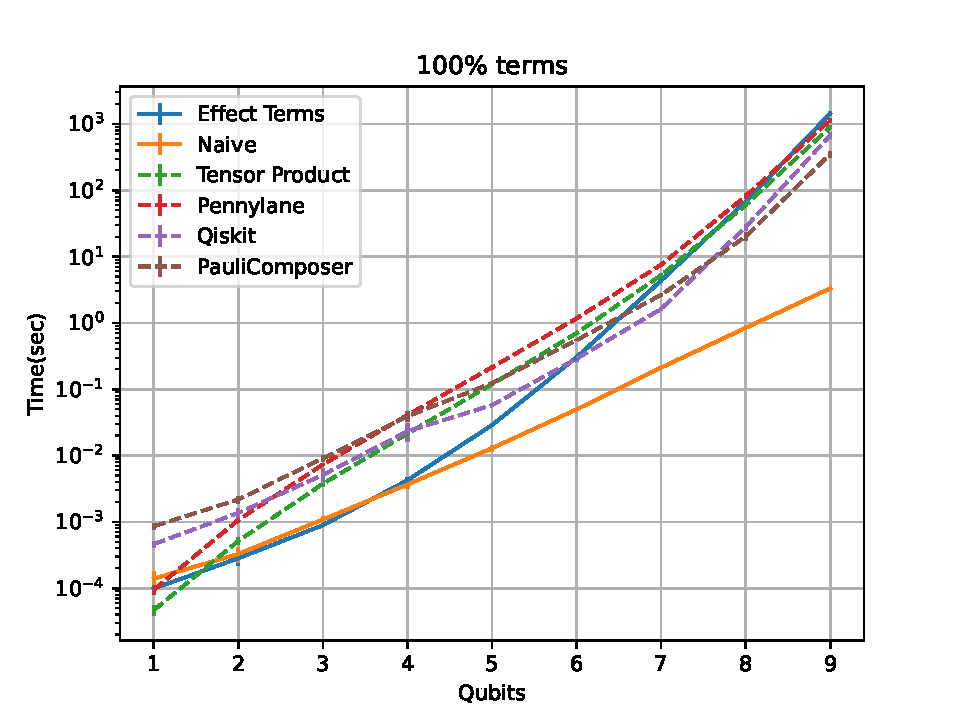
\includegraphics[width=0.7\textwidth]{media/1_terms.pdf}
    \caption{Benchmarks for matrix composition of Puali polynomials with the algorithm 1, 2 with Qiskit, Pennylane,
    PauliComposer, and standard tensor product methods, for $n = 1$ to $n = 9$. The percentages of the each case represents
    how many coefficients are non-empty in $4^n$ number of spaces.}
    \label{fig:composition_benchmark}
\end{figure}
\chapter{Miscellaneous Mathematics}

\section{Tensor Product}

\begin{definition}{\textbf{Tensor product}}
    The given two vector space, $V$ and $W$ over the field $\mathbb{F}$,
    a tensor product is a bi-linear mapping with notation, $\otimes$, such that

    \begin{equation}
        \otimes: V \times W \rightarrow \mathcal{U} = V \otimes W
    \end{equation}
\end{definition}

The generated space $\mathcal{U} = V \otimes W$ also be a 
vector space over field $\mathbb{F}$. The tensor product generates a larger vector space 
with two-given vector spaces. 

\begin{theorem}{\textbf{Properties of Tensor producted space}}

    \begin{itemize}
        \item Tensor product of the spanning sets of the each VS is a spanning set of the producted space.
        \item For finite VS $\dim(V) = n, \dim(W) = m$, $\dim(V \otimes W) = n \cdot m$.
        \item Dual space of the tensor producted space is a tensor product of dual spaces of each VS.
    \end{itemize}
\end{theorem}

In matrix space, $\mathbf{M}_{}(\mathbb{C})$ is form a Hilbert-space with Hilbert-Schmidt inner product.

\begin{definition}{\textbf{Hilbert-Schmidt Inner Product}}
    For the given two matrices, $A, B$, their inner product is defined as 

    \begin{equation}
        \langle A | B \rangle = \mbox{Tr}(A^\dagger B)
    \end{equation}
    
\end{definition}

A typical tensor product of matrix space is a \textit{Kronecker product}.

\begin{definition}{\textbf{Kronecker Product}}
    \begin{equation}
        A \otimes B = \begin{pmatrix}
            a_{11} B & \cdots & a_{1m} B\\
            \vdots & \ddots & \vdots \\
            a_{n1} B & \cdots & a_{nm} B
        \end{pmatrix}
    \end{equation}
\end{definition}

\section{Tensor product representation of quantum circuit}




\section{Lie-algebra}
Lie-group and Lie-algebra is a mathematical formulation to express the group sturcture in VS for a convience.


\chapter{NP-problems}

\section{Traveling Purchaser problem}

\subsection{Traveling Saleman problem}

\section{Max-clique Problem}
\label{appendix:max-clique}
Graph.

complment graph.

Additional topic: time evolution operator of Hamiltonian,


\printindex

\end{document}